
\chapter[Unbalanced Co-Optimal Transport]{Unbalanced Co-Optimal Transport}
\label{chap:ucoot}

\renewcommand{\contentsname}{Contents}
\localtableofcontents*
\chaptermark{\textbf{Unbalanced Co-Optimal Transport}}

\hfill \break

\raggedbottom

% This chapter presents three contributions to the unbalanced OT-based divergences,
% namely the unbalanced OT, unbalanced Co-Optimal Transport and unbalanced Gromov-Wasserstein.

% The first contribution is an ongoing work on an alternative solver for the entropic UOT problem
% \ref{eq:discrete_ent_uot}, which has not yet been studied in the literature,
% to the best of our knowledge.
% We called this approach \textit{INexact Proximal Unbalanced optimal Transport} (INPUT),
% since it is a straightforward application of the inexact Bregman Proximal Point (BPP) algorithm
% to the UOT problem. We present the derivation of INPUT, then illustrate how
% it can overcome the limitations of the MM and Sinkhorn-based methods,
% while being orders of magnitude faster in our toy experiments. Despite the simplicity,
% its convergence analysis remains a challenging open problem and is under our active research.

This chapter summarizes the results from the paper \citep{Tran23} and addresses
the unbalaced extension of Co-Optimal transport.
Optimal transport (OT) compares probability distributions by computing a meaningful alignment
between their samples. Co-optimal transport (COOT) takes this comparison further
by inferring an alignment between features as well. While this approach leads to
better alignments and generalizes both OT and Gromov-Wasserstein distances,
we provide a theoretical result showing that it is sensitive to outliers
that are omnipresent in real-world data. This prompts us to propose unbalanced COOT
for which we provably show its robustness to noise in the compared datasets.
To the best of our knowledge, this is the first such result for OT methods in incomparable spaces.
With this result in hand, we provide empirical evidence of this robustness
for the challenging tasks of heterogeneous domain adaptation with and without
varying proportions of classes and simultaneous alignment of samples and features across
single-cell measurements.

%%%%%%%%%%%%%%%%%%%%%%%%%%%%%%%%%%%%%%%%%%%%%%
\section{Unbalanced Co-Optimal Transport}
%%%%%%%%%%%%%%%%%%%%%%%%%%%%%%%%%%%%%%%%%%%%%%

%%%%%%%%%%%%%%%%%%%%%%%%%%%%%%%%%%%%%%%%%%%%%%
\subsection{Introduction}
%%%%%%%%%%%%%%%%%%%%%%%%%%%%%%%%%%%%%%%%%%%%%%

The last decade has witnessed many successful applications of optimal
transport (OT) \citep{Monge81,Kanto42} in machine learning, namely in domain adaptation \citep{Courty16},
generative adversarial networks \citep{Arjovsky17}, classification \citep{Frogner15},
dictionary learning \citep{Rolet16}, semi-supervised learning \citep{Solomon14}. When the
supports of the probability measures lie in the same ground metric space, it is natural to use the distance defined by the metric
to induce the cost, which leads to the famous Wasserstein distance \citep{Villani03}. When they do not, one can rely on the idea of Gromov-Hausdorff distance \citep{Gromov81} and its equivalent reformulations \citep{Gromov99,Kalton99,Burago01}, and adapt them to the setting of metric measure spaces \citep{Gromov99}. This results in, for example, the Gromov-Wasserstein
(GW) distance \citep{Memoli07,Memoli11,Sturm12}, which has been widely used in many applications, namely in shape matching \citep{Memoli11},
comparing kernel matrices \citep{Peyre16}, graphs \citep{Vayer19b,Xu19,Xu19b},
computational biology \citep{Demetci22}, heterogeneous domain adaptation \citep{Yan18},
correspondence alignment \citep{Solomon16}, machine translation \citep{Melis18}.

By construction, the GW distance can only provide the sample alignment that best preserves the intrinsic geometry of the distributions and, as such, compares square pairwise relationship matrices. The CO-Optimal transport (COOT) \citep{Redko20,Chowdhury21b} goes beyond these limits by simultaneously learning two independent (feature and sample) correspondences, and thus provides greater flexibility over the GW distance in terms of usage and interpretability. First, it allows us to measure similarity between arbitrary-size matrices. An interesting use case is, for instance, on tabular data, which are usually expressed as a matrix whose rows represent samples and columns represent features. For the GW distance,
the similarity or distance matrix (or any square matrix derived from the data)
must be calculated in advance and the effect of the individual variables is lost during this computation. On the other hand, COOT can bypass this step as it can use either the tabular data directly or the similarity matrices as inputs. Second, COOT provides both sample and feature correspondences. These feature correspondences are also interpretable and allow to recover relations between the features of two different datasets even when they do not lie in the same space.

Similar to classical OT, COOT enforces hard constraints on the marginal distributions
both between samples and features. These constraints lead to two main limitations:
(1) imbalanced datasets where samples or features are re-weighted
cannot be accurately compared; (2) mass transportation \emph{must} be exhaustive:
outliers, if any, must be matched regardless of the cost they induce.
To circumvent these limitations, we propose to relax the mass preservation constraints
in the COOT distance and study a broadly applicable and general OT framework
that includes several well-studied cases presented in \Cref{t:ucoot_comparisons}.

\paragraph{Related work.}
To relax the OT marginal constraints, a straightforward solution is to control
the difference between the marginal distributions of the transportation plan
and the data by some discrepancy measure, e.g., Kullback-Leibler divergence.
In classical OT, this gives rise to the unbalanced OT (UOT),
which was first proposed by \citet{Benamou03}.
The theoretical and numerical aspects of this extension
have been studied extensively \citep{Liero18,Chizat18b,Chizat18a,Khiem20}
and are gaining increasing attention in the machine
learning community, with wide-range applications, namely in
domain adaptation \citep{Fatras21}, generative adversarial networks
\citep{Balaji20, Yang19}, dynamic tracking \citep{Lee19}, crowd counting \citep{Ma21},
neuroscience \citep{janati2019group, bazeille2019} or
modeling cell developmental trajectories \citep{Schiebinger19}.

Unbalanced OT and its variants are usually sought for
their known robustness to outliers \citep{Mukherjee21,Balaji20,Fatras21}.
This appealing property goes beyond classical OT. For instance,
to compare signed and non-negative measures in incomparable spaces,
unbalanced OT \citep{Liero18} can be blended with the
$L_p$-transportation distance \citep{Sturm06}, which leads to the
Sturm-Entropic-Transport distance \citep{Ponti20}, or with the GW distance,
which gives rise to the unbalanced GW (UGW) distance \citep{Sejourne20}.
Also motivated by the unbalanced OT, \citet{Zhang21} proposed a relaxation of the
bidirectional Gromov-Monge distance called unbalanced bidirectional Gromov-Monge divergence.
\begin{table}[t]
  \small
	\centering
  \begin{tabular}{l *4c}
    \toprule
    & Across spaces & Sample alignment & Feature alignment & \makecell{Robust to outliers} \\
    \midrule
    OT & \nomark & \yesmark & \nomark & \nomark \citep{Fatras21} \\
    UOT & \nomark & \yesmark & \nomark & \yesmark \citep{Fatras21} \\
    GW & \yesmark & \yesmark & \nomark & \nomark (Prop. \ref{prop:coot_not_robust}) \\
    UGW & \yesmark & \yesmark & \nomark & \yesmark (Thm. \ref{thm:ucoot_robust}) \\
    COOT & \yesmark & \yesmark & \yesmark & \nomark (Prop. \ref{prop:coot_not_robust}) \\
    UCOOT & \yesmark & \yesmark & \yesmark & \yesmark (Thm. \ref{thm:ucoot_robust}) \\
    \bottomrule
    \hline
  \end{tabular}
  \caption{Properties of different OT formulations generalized by UCOOT.
  The proposed UCOOT is not only able to learn informative feature alignments,
  but also robust to outliers.
  \label{t:ucoot_comparisons}}
\end{table}

\paragraph{Contributions.} In this work, we introduce an unbalanced extension of COOT
called ``Unbalanced CO-Optimal transport'' (UCOOT). UCOOT -- defined for both discrete and
continuous data -- is a general framework that encompasses all the OT variants displayed
in \Cref{t:ucoot_comparisons}. Our main contribution is to show that UCOOT is provably robust
to both samples and features outliers, while its balanced counterpart can be made
arbitrarily large with strong enough perturbations. To the best of our knowledge,
this is the first time such a general robustness result is established for OT across different spaces.
Our theoretical findings are showcased in unsupervised heterogeneous domain adaptation
and single-cell multi-omic data alignment, demonstrating a very competitive performance.

\paragraph{Notations.} For any integer $n \geq 1$, we write $[n] := \{1,...,n\}$.
Given a Polish space $X$, we denote $\cM^+(X)$ the set of nonnegative and finite Borel
measures over $X$. For any $\mu \in \cM^+(X)$, we denote
its mass by $m(\mu) := \mu(X)$.
Unless specified otherwise, we always consider fully supported measures,
i.e. $\text{supp}(\mu) = X$, for any measure $\mu \in \cM^+(X)$.
The product measure of two measures $\mu$ and $\nu$ is defined as:
$d (\mu \otimes \nu)(x,y) := d\mu(x) d\nu(y)$.
Given $\pi \in \cM^{+}(X \times Y)$, we denote
$(\pi_{\#1}, \pi_{\#2})$ its marginal distributions i.e. $d\pi_{\#1} = \int_{Y} d\pi$ and
$d\pi_{\#2} = \int_{X} d\pi$.
For $\mu, \nu \in \cM^+(X)$, the Kullback-Leibler divergence is defined by
$\kl(\mu|\nu) := \int \frac{d \mu}{ d \nu} \log \frac{d \mu}{ d \nu} \mathrm d\nu
- \int \mathrm d\mu + \int \mathrm d\nu$ if $\mu \ll \nu$ and set to $+\infty$ otherwise.
Finally, the indicator divergence $\iota_{=}(\mu | \nu)$ is equal to 0 if $\mu = \nu$
and $+\infty$ otherwise.

%%%%%%%%%%%%%%%%%%%%%%%%%%%%%%%%%%%%%%%%%%%%%%%%%%

%%%%%%%%%%%%%%%%%%%%%%%%%%%%%%%%%%%%%%%%%%%%%%%
\subsection{From COOT to Unbalanced Co-Optimal Transport} \label{sec:ucoot}
The ultimate goal behind the CO-Optimal Transport (COOT)
framework is the simultaneous alignment of samples \emph{and} features to allow for
comparisons across spaces of different dimensions. In this section, we discuss
OT formulations including OT, UOT, GW, UGW and COOT, then introduce the proposed UCOOT
and show how the aforementioned distances fall into our framework.

% \iffalse After some examples, we present our main theoretical contribution:the robustness to sample and feature outliers. \fi

\paragraph{From sample alignment to sample-feature alignment.}
Let $(X_1^s, \mu_1^s)$ and $(X_2^s, \mu_2^s)$ be a pair of compact measure spaces such that
$X_1^s$ and $X_2^s$ belong to some common metric space $(\cE, d)$.
Classical (unbalanced) optimal transport infers one alignment (or joint distribution)
$\pi^s \in \cM^+(X_1^{s} \times X_2^s)$ with marginals $(\pi^{s}_{\#1}, \pi^{s}_{\#2})$
close to $(\mu_1^s, \mu_2^s)$ according to some appropriate divergence $D$ such that
the cost $\int c(x_1, x_2) \; \mathrm d\pi^{s}(x_1, x_2) + D(\pi^{s}_{\#1} | \mu_1^s)
+ D(\pi^{s}_{\#2} | \mu_2^s)$ is minimal. For instance, in balanced (resp. unbalanced) OT,
$D$ corresponds to the indicator divergence (resp. KL divergence or TV).
To define a generalized OT beyond one single alignment, we must first introduce
a new pair of measure spaces $(X_1^{f}, \mu_1^f)$ and $(X_2^{f}, \mu_2^f)$.
Intuitively,  the two transport plans that must be inferred: $\pi^s$ across \emph{samples}
and $\pi^f$ across \emph{features}, must minimize a cost of the form
$\iint c((x_1^s, x_1^f), (x_2^s, x_2^f)) \; \mathrm d\pi^s(x_1^s, x_2^s)\; \mathrm d \pi^f(x_1^f, x_2^f)$
where $c((x_1^s, x_1^f), (x_2^s, x_2^f))$ is the \emph{joint} cost of aligning
the sample-feature pairs $(x_1^s, x_1^f)$ and $(x_2^s, x_2^f)$.

However, unlike OT,
there is no underlying ambient metric space in which comparisons between these pairs
are straightforward. Thus, we consider a simplified cost of the form:
$c((x_1^s, x_1^f), (x_2^s, x_2^f)) = |\xi_1(x_1^s, x_1^f) - \xi_2(x_2^s, x_2^f)|^p$, for $p \geq 1$
and some scalar functions $\xi_1, \xi_2$ that define the sample-feature interactions.
A similar definition was adopted by \citet{Chowdhury21b} to extend COOT to the continuous setting
in the context of hypergraphs. Formally, our general formulation takes
pairs of \emph{sample-feature spaces} defined as follows.

\begin{definition}[Sample-feature space]
Let $(X^s, \mu^s)$ and $(X^f, \mu^f)$ be compact Polish measure spaces, where $\mu^f \in \cM^+(X^f)$
and $\mu^s \in \cM^+(X^s)$. Let $\xi$ be a scalar integrable function in
$L^p(X^s \times X^f, \mu^s \otimes \mu^f)$. We call the triplet
$\cX = ((X^s, \mu^s), (X^f, \mu^f), \xi)$ a sample-feature space and $\xi$ is called an interaction.
\end{definition}
%
%%%%%%%%%%%%%%%%%%%%%%%%%%%%%%%%%%%%%%%%%%%%%%%%
\begin{definition}[Generalized COOT]
\label{def:ucoot}
Given two divergences $D_1$ and $D_2$, we define the generalized COOT of order $p$
between $\cX_1 = ((X_1^s, \mu_1^s), (X_1^f, \mu_1^f), \xi_1)$ and
$\cX_2 = ((X_2^s, \mu_2^s), (X_2^f, \mu_2^f), \xi_2)$ by:
\begin{equation}
\label{eq:ucoot}
  \begin{split}
  \inf_{\substack{\pi^s \in \cM^+(X_1^s \times X_2^s) \\
  \pi^f \in \cM^+(X_1^f \times X_2^f) \\ m(\pi^s) = m(\pi^f)}}
  &\underbrace{\iint |\xi_1(x_1^s, x_1^f) - \xi_2(x_2^s, x_2^f)|^p
  \; \mathrm d\pi^s \; \mathrm d \pi^f}_{\text{transport cost of sample-feature pairs}}
  + \underbrace{\sum_{k=1}^2\rho_k D_k(\pi^s_{\#k} \otimes \pi^f_{\#k} |
  \mu^s_k \otimes \mu^f_k)}_{\text{mass destruction / creation penalty}},
  \end{split}
\end{equation}
for $\rho_1, \rho_2 >0$ and $p \geq 1$.
\end{definition}
As the multiplicative nature between $\pi^s$ and $\pi^f$ leads to an invariance by the scaling map
$\alpha \mapsto (\alpha \pi^s, \frac{1}{\alpha} \pi^f)$, for $\alpha > 0$,
we further impose the equal mass constraint $m(\pi^s) = m(\pi^f)$.

It is worth mentioning that Formulation \eqref{eq:ucoot} is not the only way to
relax the marginal constraints. For example, instead of
$D_k(\pi^s_{\#k} \otimes \pi^f_{\#k} | \mu^s_k \otimes \mu^f_k)$,
one can consider $D_k(\pi^s_{\#k} | \mu^s_k) + D_k( \pi^f_{\#k} | \mu^f_k)$,
or $D_s(\pi^s_{\#1} \otimes \pi^s_{\#2} | \mu^s_1 \otimes \mu^s_2)$,
for some divergence $D_s$. However, amongst these choices,
ours is the only one which can be recast as a variation of the unbalanced OT problem.
This allows us to leverage the known techniques in unbalanced OT to justify
the theoritical and practical properties, namely \Cref{prop:existence}
and \Cref{thm:ucoot_robust} below.

Note that the problem above is very general and can, with some additional
constraints, recover exact OT, UOT, GW, UGW, COOT (see \Cref{t:examples}).
In particular, if the measures $(\mu^s_1, \mu^s_2)$ and $(\mu^f_1, \mu^f_2)$
are probability measures, then setting $D_1 = D_2 = \iota_=$ leads to the
COOT problem first introduced in the discrete case in \citep{Redko20} and
recently generalized to the continuous setting in \citep{Chowdhury21b}
\footnote{Note that, \citet{Chowdhury21b} consider \textbf{bounded measurable} function
on the Polish measure space, whereas we work with \textbf{integrable} function
on the \textbf{compact} Polish measure space.}
In this work, we relax the hard constraints and consider a more flexible formulation
with the KL divergence:
\begin{definition}[UCOOT]
   We define Unbalanced COOT (UCOOT) as in \Cref{eq:ucoot} with $D_1 = D_2 = \kl$.
   We write $\ucoot_{\rho}(\cX_1, \cX_2)$ to indicate the UCOOT between
   two sample-feature spaces $\cX_1$ and $\cX_2$, for a given
   pair of hyperparameters $\rho = (\rho_1, \rho_2)$.
\end{definition}
While various properties of the divergences $D_k$ have been extensively studied
in the context of unbalanced OT by several authors \citep{Chizat17,Frogner15},
the concept of sample-feature interaction requires more clarification.
Let us consider some simple examples.
In the discrete case, we consider $n$ observations of $d$ features
represented by matrix $A \in \bbR^{n \times d}$. In this case, the space $X^s$ (resp. $X^f$)
is not explicitly known but can be characterized by the finite set $[n]$ (resp. $[d]$),
up to an isomorphism. Assuming that all samples (resp. features) are equally important,
the discrete empirical measures can be given by uniform weights $\mu^s = \frac{1_{n}}{n}$
(resp. $\mu^f = \frac{1_{d}}{d}$). The most natural sample-feature interaction $\xi$ is simply
the index function $\xi(i, j) = A_{ij}$. In the continuous case,
we assume that data stream from a continuous random variable $a \sim \mu_s \in \cP(\bbR^d)$
for which an interaction function can be $\xi(a, j) = a_j$.
\begin{table}[t]
  \centering
  \small
  \begin{tabular}{l *4c}
      \toprule
          & Shape of inputs & Coupling constraint & Scalar function & Divergence \\
      \midrule
      OT   & $d_1 = d_2$              & $\pi^f = I_{d_1} = I_{d_2}$ & $\xi(i, j) = A_{ij}$                        & $\iota_=$ \\
      GW   & $n_1 = d_1$, $n_2 = d_2$ & $\pi^f = \pi^s$             & $\xi(i, j) = \text{dist}( A_{i.}, A_{j.} )$ & $\iota_=$ \\
      COOT & --                       & --                          & $\xi(i, j) = A_{ij}$                        & $\iota_=$ \\
      semi-d. COOT & --               & --                          & $\xi(a, j) = a_j$                           & $\iota_=$ \\
      UCOOT & --                      & --                          & $\xi(i, j) = A_{ij}$                        & KL \\
        \bottomrule
        \hline
        \end{tabular}
        \caption{Conditions under which different OT formulations fall within
        the generalized framework of \Cref{def:ucoot}.
        ``semi-d'' refers to ``semi-discrete'' setting, where
        $\mu_s$ is a continuous probability and $\mu_d = 1_d/d$.
        Here, $I_d$ is the identity matrix in $\bbR^d$.
  \label{t:examples}}
\end{table}
\begin{proposition} \label{prop:existence}
For any $D_1$, $D_2 \in \{ \iota_{=}, \kl \}$, Problem \eqref{def:ucoot} (in Equation \eqref{eq:ucoot})
admits a minimizer.
\end{proposition}

\begin{remark}
The existence of minimizer shown in \Cref{prop:existence}
can be extended to a larger family of Csiszár divergences \citep{Csiszar63}.
A general proof is given in the Appendix.
\end{remark}

\paragraph{Relation between UCOOT and COOT.} When $ \mu^s_k$ and $\mu^f_k$ are probability measures,
for $k=1,2$, then $\ucoot_{\rho}(\cX_1, \cX_2) \leq \coot(\cX_1, \cX_2)$,
for any $\rho_1, \rho_2 > 0$.
Moreover, $\ucoot_{\rho}(\cX_1, \cX_2) = 0$ if and only if $\coot(\cX_1, \cX_2) = 0$.
In particular, suppose that $\cX_1$ and $\cX_2$ are two finite sample-feature spaces
such that $(X^s_1, X^s_2)$ and $(X^f_1, X^f_2)$ have the same cardinality and
are equipped with the uniform measures $\mu_1^s = \mu_2^s$, $\mu_1^f = \mu_2^f$.
Then $\ucoot_{\rho}(\cX_1, \cX_2) = 0$ if and only if
there exist perfect alignments between rows (samples) and between
columns (features) of the interaction matrices $\xi_1$ and $\xi_2$.

\paragraph{Relation between UCOOT and its solution.}
UCOOT is a quadratic function of its minimizer, thanks to the property of the
KL divergence. More precisely, if $(\pi_*^s, \pi_*^f)$ is the equal-mass solution,
then by using the proof technique of Lemma 4 in \citep{Khiem20}, one can show that
\begin{align}
  \label{eq:ucoot_minimizer_minimum}
  \ucoot_{\rho}(\cX_1, \cX_2) =
  \sum_{k=1, 2} \rho_k \; m(\mu_k^s) \; m(\mu_k^f) - (\rho_1  + \rho_2) \; m(\pi^s_*)^2.
\end{align}

\subsection{Robustness of Unbalanced Co-Optimal Transport} \label{sec:robustness}
When discussing the concept of robustness, outliers are often considered as samples
not following the underlying distribution of the data. In our general context of
sample-feature alignments, we consider a \emph{pair} $(x^s, x^f) \in X^s \times X^f$
to be an outlier if the magnitude of $|\xi(x^s, x^f)|$ is abnormally larger than
other interactions between $X^s$ and $X^f$. As a result, such outliers lead to
abnormally large transportation costs $|\xi_1 - \xi_2|$. To study the robustness of COOT and UCOOT,
we consider an outlier scenario where the marginal data distributions are contaminated
by some additive noise distribution.
\begin{assumption}
\label{assump:robust}
Consider two sample-feature spaces $\cX_1$ and $\cX_2$.
Let $\varepsilon^s$ (resp. $\varepsilon^f$) be a probability measure with
compact support $O^s$ (resp. $O^f$). For $a \in \{s, f\}$,
define the noisy distribution $\widetilde{\mu}^a = \alpha_a \mu^a + (1-\alpha_a) \varepsilon^a$,
where $\alpha_a \in [0,1]$. We assume that $\xi_1$ is defined on
$(X^s_1 \cup O^s) \times (X^f_1 \cup O^f)$ and
that $\xi_1, \xi_2$ are continuous on their supports.
We denote the contaminated sample-feature space by
$\widetilde{\cX_1} = ((X^s_1 \cup O^s, \widetilde{\mu}^s_1), (X^f_1 \cup O^f, \widetilde{\mu}^f_1), \xi_1)$.
Finally, we define some useful minimal and maximal costs:
  \begin{equation}
    \begin{cases}
  \Delta_{0} := \min\limits_{
  \substack{
       x_1^s \in O^s, x_1^f \in O^f  \\
       x_2^s \in X_2^s, x_2^f \in X_2^f
  }}\quad |\xi_1(x_1^s, x_1^f) - \xi_2(x_2^s, x_2^f)|^p \\
  \Delta_{\infty} := \max\limits_{
  \substack{
  x_1^s \in X_1^s \cup O^s, x_1^f \in X_1^f \cup O^f \\
  x_2^s \in X_2^s, x_2^f \in X_2^f
  }} \quad|\xi_1(x_1^s, x_1^f) - \xi_2(x_2^s, x_2^f)|^p \enspace.
  \end{cases}
  \end{equation}
Here, $\Delta_{0}$ accounts for the minimal deviation of the cost between
the outliers and target support, while $\Delta_{\infty}$ is the maximal deviation
between the contaminated source and the target.
\end{assumption}
The exact marginal constraints of COOT enforce conservation of mass.
Thus, outliers \emph{must} be transported no matter how large their transportation costs are.
This intuition is captured by the following result.
%%%%%%%%%%%%%%%%%%%%%%%%
\begin{proposition}[COOT is sensitive to outliers]
Consider $\widetilde{\cX_1}, \cX_2$ as defined in \Cref{assump:robust}.
Then
\label{prop:coot_not_robust}
\begin{equation}
    \coot(\widetilde{\cX_1}, \cX_2) \geq (1 - \alpha_s)(1-\alpha_f)\Delta_0.
\end{equation}
\end{proposition}
%%%%%%%%%%%%%%%%%%%%%%%%
Whenever the outlier proportion $(1-\alpha_s)(1-\alpha_f)$ is positive,
COOT increases with the distance between the supports of the outliers and those of the clean data.
Thus, the right hand side of \Cref{prop:coot_not_robust} can be made arbitrarily
large by taking outliers far from the supports of the clean data.

We can now state our main theoretical contribution.
Relaxing the marginal constraints leads to a loss that saturates
as outliers get further from the data:
\begin{theorem}[UCOOT is robust to outliers]
\label{thm:ucoot_robust}
Consider two sample-feature spaces $\widetilde{\cX_1}, \cX_2$ as defined
in \Cref{assump:robust}. Let $\delta := 2(\rho_1 + \rho_2)(1 - \alpha_s\alpha_f)$
and $K = M + \frac{1}{M}\ucoot(\cX_1, \cX_2) +\delta$,
where $M= m(\pi^s) = m(\pi^f)$ is the transported mass between clean data. Then:
\begin{align} %\label{eq:ucoot-robust}
  \ucoot(\widetilde{\cX_1}, \cX_2)
  &\leq \alpha_s \alpha_f \ucoot(\cX_1, \cX_2)
  + \delta M \left[ 1 - \exp \left( {- \frac{\Delta_{\infty}(1+M) + K}{\delta M}} \right) \right].
\end{align}
\end{theorem}
%%%%%%%%%%%%%%%%%%%%%%%%%%%%%%%%%%%%%%%%%
The proof of \Cref{thm:ucoot_robust} is provided in the Appendix and
inspired from \citep{Fatras21}, but in a much more general setting:
(1) it covers both sample and feature outliers and
(2) considers a noise distribution instead of a Dirac.
Note that the bound in \Cref{prop:coot_not_robust}
indicates that outliers can make COOT arbitrary large,
while UCOOT is upper bounded and discards the mass of outliers with high transportation cost.

\setlength{\columnsep}{10pt}%
\setlength{\intextsep}{0pt}
\begin{wrapfigure}[10]{r}{0.4\textwidth}
  \centering
  \vspace{-10pt}
  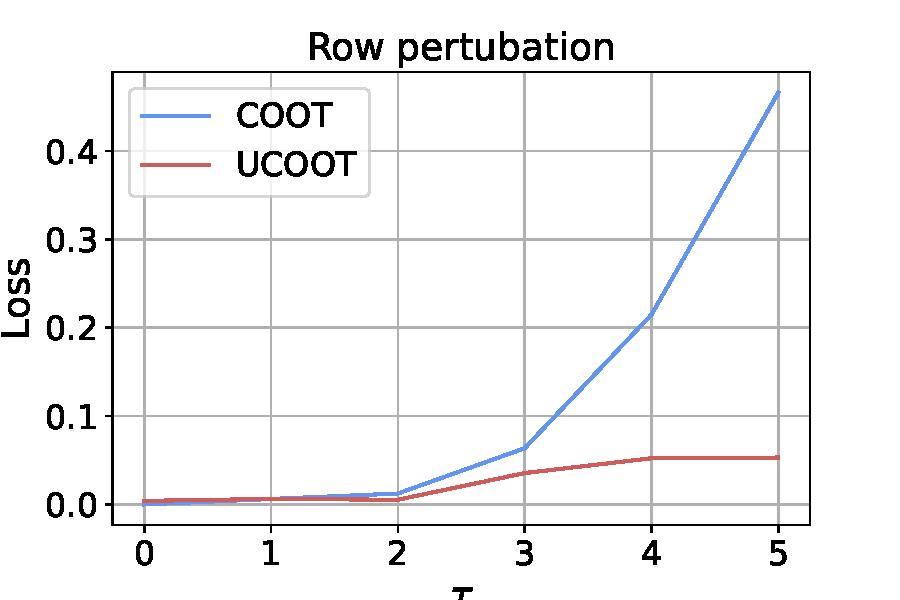
\includegraphics[width=\linewidth]{./Chapitre3/fig/robustness_2.pdf}
  \caption{Sensitivity of COOT and UCOOT under the presence of outliers.
  \label{fig:robust}}
% \end{figure}
\end{wrapfigure}
This is well illustrated in \Cref{fig:robust},
where we simulate outliers by adding a perturbation to a row of the interaction matrix.
More precisely, we first generate a matrix $A \in \mathbb R^{20 \times 15}$ by
$A_{ij} = \cos(\frac{i}{20} \pi) + \cos(\frac{j}{15} \pi)$.
Then, we replace its last row by $\tau 1_{15}$, for $\tau \geq 0$.
\Cref{fig:robust} depicts COOT and UCOOT between $A$
and its modified version as a function of $\tau$. The higher the value of $\tau$,
the more likely that the last row contains the interaction of outliers.
Consequently, as $\tau$ increases, so does COOT but at a much higher pace,
whereas UCOOT remains stable.

It should be noted that, with minimal adaptation, \Cref{thm:ucoot_robust}
also holds for the unbalanced GW (UGW) distance.
This provides a theoretical explanation of the empirical observation in \citep{Sejourne20}
that unlike GW, the UGW distance is also robust to outliers.

%%%%%%%%%%%%%%%%%%%%%%%%%%%%%%%%%%%%%%%%%%%%%%%%
\subsection{Optimization algorithm and complexity} \label{subsec_app:algo}
%%%%%%%%%%%%%%%%%%%%%%%%%%%%%%%%%%%%%%%%%%%%%%%%
Solving COOT-type problems, in general, is not trivial. As highlighted in \citep{Redko20},
the balanced case corresponds to a convex relaxation of the bilinear assignment problem,
which seeks the pair of permutations minimizing the transport cost.
Here we argue that relaxing the marginal constraints makes the problem easier
in two different aspects: (1) the obtained problem is easier to solve
through a sequence of GPU friendly iterations; (2) regularization leads to lower alignment costs
and thus better local minima. In this section, we first describe how to compute UCOOT in practice.

\paragraph{Optimization strategy}
We consider two tabular datasets $A \in \bbR^{n_1 \times d_1}$ and $B \in \bbR^{n_2 \times d_2}$.
Let $u_k$ be the uniform histogram over sample-feature pairs:
$u_k := \frac{1}{n_kd_k}1_{n_k} \otimes 1_{d_k}$, for $k=1, 2$.
For the sake of simplicity, we assume uniform weights over both samples and features.
Computing UCOOT can be done using block-coordinate descent (BCD) both with
and without entropy regularization. More precisely, given a hyperparameter $\varepsilon \geq 0$,
discrete UCOOT can be written as:
\begin{equation}
\begin{split}
    \label{eq:ucoot-discrete-2}
  &\min_{\substack{\pi^s, \pi^f \\
  \iffalse \in \bbR_+^{n_1, n_2} \\ \pi^f \in \bbR_+^{d_1, d_2} \\ \fi m(\pi^s) = m(\pi^f)}}
  \sum_{i, j, k, l} (A_{ik} - B_{jl})^2\pi^s_{ij}\pi^f_{kl} +
  \rho_1 \kl(\pi^s 1_{n_1} \otimes \pi^f 1_{d_1} | u_1 )  \\
  &+ \rho_2 \kl({\pi^s}^\top 1_{n_2} \otimes {\pi^f}^{\top} 1_{d_2} | u_2) +
  \varepsilon \text{KL}( \pi^s \otimes \pi^f | \mu^s_1 \otimes \mu_2^s \otimes \mu_1^f \otimes \mu_2^f).
\end{split}
\end{equation}

\begin{algorithm}[t]
    \caption{BCD algorithm to solve UCOOT \label{alg:bcd}}
    \begin{algorithmic}
      \STATE {\bfseries Input:} $A \in \bbR^{n_1, d_1}, B \in \bbR^{n_2, d_2}$, $\rho_1, \rho_2, \varepsilon$
      \STATE Initialize $\pi^s$ and $\pi^f$
      \REPEAT
      \STATE Update $\pi^s$ using Sinkhorn or MM
      \STATE Rescale $\pi^s = \sqrt{\frac{m(\pi^f)}{m(\pi^s)}} \pi^s$
      \STATE Update $\pi^s$ using Sinkhorn or MM
      \STATE Rescale $\pi^f = \sqrt{\frac{m(\pi^s)}{m(\pi^f)}} \pi^f$
      \UNTIL{convergence}
	\end{algorithmic}
\end{algorithm}
The only difference between $\varepsilon = 0$ and $\varepsilon > 0$
lies in the inner-loop algorithm used to update one of transport plans $(\pi^s, \pi^f)$
while the other one remains fixed.
For $\varepsilon=0$, we use the Majorization-Minimization (MM) algorithm \citep{Chapel21},
which leads to a multiplicative update on the transport plan.
For $\varepsilon > 0$, updating each transport plan boils down to an entropic UOT problem,
which can be solved efficiently using the unbalanced variant of Sinkhorn's algorithm \citep{Chizat18a}.
The main benefit of entropy regularization is to reduce the number of variables
from $(n_1 \times n_2) + (d_1 \times d_2)$ to $n_1 + n_2 + d_1 + d_2$.
Moreover, by taking $\varepsilon$ sufficiently small, we can recover solutions
close to those in the non-entropic case. We formalize this claim in the following result.
%%%%%%%%%%%%%%%%%%%%%%%%%%%%%%%%%%%%%%%%%%
\begin{proposition}
  \label{prop:convergence_minimiser_unbalanced}
  Let $(\pi_{\varepsilon}^s, \pi_{\varepsilon}^f)$ be an equal-mass solution of the problem
  $\ucoot_{\rho, \varepsilon}(\cX_1, \cX_2)$. Denote $\mu^s = \mu_1^s \otimes \mu_2^s$
  and $\mu^f = \mu_1^f \otimes \mu_2^f$.
  \begin{enumerate}
    \item When $\varepsilon \to \infty$, we have $\pi_{\varepsilon}^s \rightharpoonup
    \sqrt{\frac{m(\mu^f)}{m(\mu^s)}} \mu^s$
    and $\pi_{\varepsilon}^f \rightharpoonup \sqrt{\frac{m(\mu^s)}{m(\mu^f)}} \mu^f$.

    \item When $\varepsilon \to 0$, we have
    \begin{enumerate}
      \item $\ucoot_{\rho, \varepsilon}(\cX_1, \cX_2) \to \ucoot_{\rho}(\cX_1, \cX_2)$ and
      $m(\pi_{\varepsilon}^s) \to m(\pi_*^s)$, for any equal-mass solution
      $(\pi_*^s, \pi_*^f)$ of the unregularized problem.

      \item Any cluster point $(\widehat{\pi}^s, \widehat{\pi}^f)$ of the sequence
      $(\pi_{\varepsilon}^s, \pi_{\varepsilon}^f)_{\varepsilon}$ is an equal-mass
      solution of the unregularized problem. Furthermore,
      \begin{equation}
        \kl(\widehat{\pi}^s \otimes \widehat{\pi}^f | \mu^s \otimes \mu^f) =
        \min_{(\pi^s, \pi^f)} \kl(\pi^s \otimes \pi^f \vert \mu^s \otimes \mu^f),
      \end{equation}
      where the infimum is taken over all solutions of the unregularized problem.
    \end{enumerate}
  \end{enumerate}
\end{proposition}

%%%%%%%%%%%%%%%%%%%%%%%%%%%%%%%%%%%%%%%%%%%%%%%%
\subsection{Experiments} \label{sec:experiments}
\subsubsection{Illustration and interpretation on MNIST images}

\begin{figure}[t]
  \centering
  \includegraphics[trim={0.5cm 4.5cm 1.5cm 2.4cm}, clip, width=\linewidth]{./Chapitre3/fig/mnist-ucoot-rebuttal.pdf}
  \caption{Example illustrating the feature alignment $\pi_f$ learned by UCOOT
  and its robustness to outliers.
  \textbf{(a)} Visualization of 4 random samples from both datasets.
  The added Gaussian noise only affects the first 10 columns of the images
  and is different across images.
  \textbf{(b)} The barycentric mapping (see Appendix for details)
  defined by UCOOT learns the transformation defined by $\varphi_\sigma$
  while disregarding non-informative features.
  \textbf{(c)} Alignments across samples from $X$ and $Y$.
  We contaminated the target $Y$ with 50 sample outliers
  (images with uniform entries in $[0,1]$).
  A very small amount of noise is sufficient to derail COOT.
  Unlike COOT, UCOOT does not transport any outlier sample.
  Accuracy is computed as the percentage of mass within the block-diagonal structure.
  \label{f:mnist-example}}
\end{figure}
We illustrate the robustness of UCOOT and its ability to learn meaningful feature alignments
under the presence of both sample and feature outliers in the MNIST dataset.
We introduce the feature outliers by applying a handcrafted transformation $\varphi_\sigma$
that performs a zero-padding (shift), a 45\textdegree\ rotation,
a resize to (28, 34) and adds Gaussian noise $\cN(0, \sigma^2)$ entries
to the first 10 columns of the image.

\Cref{f:mnist-example} (a) shows some examples of original and transformed images.
We randomly sample 100 images per class (1000 total) from $X = \text{MNIST}$ and
$Y = \varphi_{\sigma}(\text{MNIST})$. Regarding the sample outliers,
we add 50 random images with uniform entries in [0, 1] to the target data $Y$.
We then compute the optimal COOT and UCOOT alignments shown in
\Cref{f:mnist-example} (b) and (c).
The flexibility of UCOOT with respect to mass transportation allows it to completely disregard:
(1) noisy and uninformative pixels (features),
which are all given the same weight as depicted by (b);
(2) all the sample outliers of which none are transported as shown
by the last blank column of the alignment (c).
Moreover, notice how the color-coded input image is transformed according to
the transformation $\varphi_{\sigma}$ despite the fact that
no spatial information is provided in the OT problem. On the other hand,
a very small perturbation ($\sigma = 0.01)$ is enough for the sample alignment
given by COOT to lose its block-diagonal dominant structure (class information is lost),
while the UCOOT alignment remains unscathed.

\setlength{\intextsep}{0pt}
\begin{wrapfigure}[10]{r}{0.4\textwidth}
    \centering
    \vspace{-12pt}
    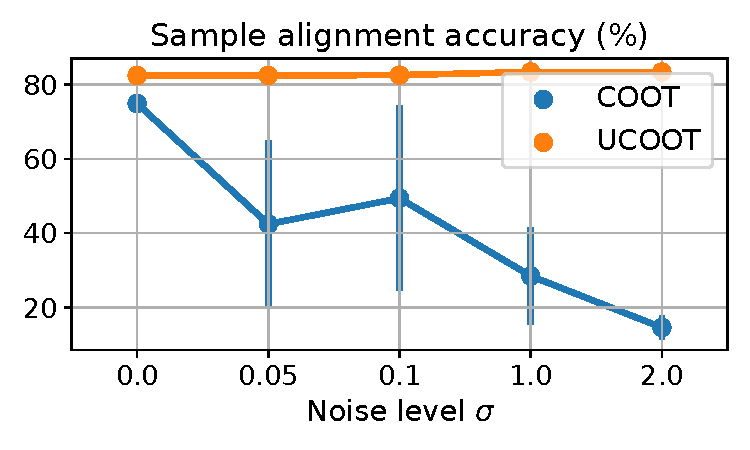
\includegraphics[width=\linewidth]{./Chapitre3/fig/mnist-sigma.pdf}
    \vspace*{-9mm}
    \caption{Robustness of UCOOT vs. COOT on MNIST example, at different noise levels.
    \label{f:mnist-sigma}}
\end{wrapfigure}
One may wonder whether the performance of UCOOT would still hold for different values of $\sigma$.
\Cref{f:mnist-sigma} answers this question positively.
For $\sigma > 0$, we compute the average accuracy
(defined by the percentage of mass within the block-diagonal structure) over 20 different runs.
The performance of COOT not only degrades with noisier outliers but is also unstable.
By contrast, the accuracy of UCOOT remains almost constant regardless of the level of noise.

\subsubsection{Heterogeneous Domain Adaptation}

%Domain adaptation (DA) refers to the problem in which a classifier
%learned on one domain (called \textit{source}) can generalise well to the other one (called \textit{target}).
We now investigate the application of discrete UCOOT in semi-supervised and unsupervised
Heterogeneous Domain Adaptation (HDA). It is a particularly difficult problem where
one aims to predict classes on unlabeled data using labeled data lying in a different space.
OT methods across spaces have recently shown good performance on such tasks,
in particular using GW distance \citep{Yan18} and COOT \citep{Redko20}.
%i.e. the samples in source and target domains live in the different spaces, and we have no access to the labelled target sample.
%It should be noted that COOT and UCOOT have already been used in real-world applications.
% For example, as the entropic GW distance and its COOT follow exactly the same approximation scheme, they share the success in
% graph matching \citep{Xu19b}, correspondance alignment \citep{Solomon16},
% comparing kernel matrices \citep{peyre16}. On the other hand, the recent discrete COOT also works well in co-clustering and
% HDA tasks \citep{Redko20} and the UCOOT has shown competitive performance in positive-unlabelled learning \citep{Sejourne20}.

\paragraph{Datasets and experimental setup.} We consider the Caltech-Office dataset \citep{Saenko10}
containing three domains:
Amazon (A) ($1123$ images), Caltech-$256$ (C) ($958$ images) and Webcam (W) ($295$ images)
with 10 overlapping classes amongst them. The image in each domain is representated by
the output of the second last layer
in the Google Net \citep{Szegedy15} and Caffe Net \citep{Jia14} neural network architectures,
which results in $4096$ and $1024$-dimensional vectors, respectively (thus $d_s = 4096, d_t = 1024$).
We compare $4$ OT-based methods: GW, COOT, UGW, and UCOOT. For the semi-supervised HDA task,
we additionally use $k$-NN, with $k=3$ as baseline method, which corresponds to the situation where
there is no adaptation. The hyper-parameters for each method are validated on a
unique pair of datasets (W$\rightarrow$W),
then fixed for all other pairs in order to provide truly unsupervised HDA generalization.

We follow the same experimental setup as in \citep{Redko20}. For each pair of domains,
we randomly choose $20$ samples per class (thus $n_s = n_t = 200$) and
perform adaptation from CaffeNet to GoogleNet features, then calculate the
accuracy of the generated predictions on the target domain using OT label propagation \citep{Redko19a}.
This technique uses the OT plan to estimate the amount of mass transported from each class
(since the sources are labeled) to a given target sample.
The predicted class corresponds to the one which contains the most mass.
% : except for the baseline, for each method, we use the learned sample coupling between source and
% target data to predict the labels in the target domain via label propagation \citep{Redko19a}.
% More precisely, for each pair of domains, we randomly choose $20$ samples per class (thus $n_s = n_t = 200$) and
% perform adaptation from CaffeNet to GoogleNet features, then calculate the accuracy of the generated predictions on the target domain.
We repeat this process $10$ times and calculate the average and standard deviation of the performance.
In both source and target domains, we assign uniform sample and feature distributions.

In the semi-supervised HDA task, we incorporate the prior knowledge on the target labels by adding an
additional cost matrix to the training of sample coupling, so that a source sample
will be penalized if it transfers mass to the target samples in the different classes.
More precisely, we introduce the masked target label $\tilde{y}^{(t)} \in \mathbb R^{n_t}$
defined by randomly keeping $\tilde{n}_t \in \{1,3,5\}$ samples in each class
in the target label $y^{(t)}$ and masking all other labels in $y^{(t)}$ by $-1$.
Then the additional cost $M \in \mathbb R^{n_s \times n_t}$ between $y^{(s)}$
and $\tilde{y}^{(t)}$ is defined by
\begin{equation}
  M_{ij} =
  \begin{cases}
    0, \text{ if } y^{(s)}_i = \tilde{y}^{(t)}_j, \text{ or } \tilde{y}^{(t)}_j = -1 \\
    v, \text{ otherwise}.
  \end{cases}
\end{equation}
Here, $v > 0$ is a fixed value and we choose $v = 100$ in this experiment.

Once the sample coupling $P$ is learned, the label propagation works as follows:
suppose the labels contain $K$ different classes,
we apply the one-hot encoding to the source label $y^{(s)}$ to obtain
$D^{(s)} \in \mathbb R^{K \times n_s}$ where $D^{(s)}_{ki} = 1_{\{y^{(s)}_i = k\}}$.
The label proportions on the target data are estimated by:
$L = D^{(s)} P \in \mathbb R^{K \times n_t}$. Then the prediction can be generated by choosing the
label with the highest proportion, i.e. $\widehat{y}^{(t)}_j = \arg\max_k L_{kj}$.
Note that, while the prediction is performed on the whole target samples,
only those whose labels are masked as $-1$ during the
training, are used in the calculation of accuracy. For the $k$-NN only,
we train a classifier on the labelled target samples, then perform prediction on the unlabelled ones.

\paragraph{HDA results.}
\begin{table}[t]
  \centering
  \small
		\begin{tabular}{c c c c c}
				\toprule
				Domains & GW & UGW & COOT & UCOOT \\
				\midrule

				C $\to$ C & 16.25 ($\pm$ 7.54) & 10.85 ($\pm$ 2.13) & 36.40 ($\pm$ 12.94) & \textbf{44.05 ($\pm$ 19.33)} \\
				\hline
				C $\to$ A & 12.95 ($\pm$ 7.74) & 11.60 ($\pm$ 4.86) & 28.30 ($\pm$ 11.78) & \textbf{31.90 ($\pm$ 7.43)} \\
				\hline
				C $\to$ W & 18.95 ($\pm$ 9.43) & 14.15 ($\pm$ 3.98) & 19.55 ($\pm$ 14.51) & \textbf{28.55 ($\pm$ 6.60)} \\
				\hline

				A $\to$ C & 16.40 ($\pm$ 8.99) & 10.25 ($\pm$ 5.66) & \textbf{41.80 ($\pm$ 14.81)} & 39.15 ($\pm$ 17.98) \\
				\hline
				A $\to$ A & 14.75 ($\pm$ 15.20) & 20.20 ($\pm$ 6.45) & \textbf{57.90 ($\pm$ 16.84)} & 42.45 ($\pm$ 15.47) \\
				\hline
				A $\to$ W & 14.55 ($\pm$ 8.83) & 20.65 ($\pm$ 4.13) & 42.10 ($\pm$ 7.80) & \textbf{48.55 ($\pm$ 13.06)} \\
				\hline

				W $\to$ C & 20.65 ($\pm$ 11.90) & 14.20 ($\pm$ 5.13) & 8.60 ($\pm$ 6.56) & \textbf{69.80 ($\pm$ 14.91)} \\
				\hline
				W $\to$ A & 17.00 ($\pm$ 9.75) & 7.10 ($\pm$ 2.45) & 16.65 ($\pm$ 10.01) & \textbf{30.55 ($\pm$ 10.09)} \\
				\hline
				W $\to$ W & 19.30 ($\pm$ 11.87) & 24.40 ($\pm$ 3.28) & \textbf{75.30 ($\pm$ 3.26)} & 51.50 ($\pm$ 20.51) \\
				\bottomrule
				Average & 16.76 ($\pm$ 10.14) & 14.82 ($\pm$ 4.23) & 36.29 ($\pm$ 10.95) & \textbf{42.94 ($\pm$ 13.93)} \\
				\bottomrule
			\end{tabular}
	\caption{Unsupervised HDA from CaffeNet to GoogleNet. \label{tab:hda}}
\end{table}

The means and standard deviations of the accuracy on target data are reported in \Cref{tab:hda}
for all the methods and all pairs of datasets. We observe that, thanks to its robustness,
UCOOT outperforms COOT on 7 out of 9 dataset pairs, with higher average accuracy
but also slightly larger variance. This is because of the difficulty of the
unsupervised HDA problem and the instability present in all methods. In particular,
GW-based approaches perform very poorly. This may be due to the fact that the
pre-trained models contain meaningful but a very high-dimensional vectorial representation
of the image. Thus, using the Euclidean distance matrices as inputs not only causes
information loss but also is less relevant (see for example, \citep{Aggarwal01},
or Theorem 3.1.1 and Remark 3.1.2 in \citep{Vershynin18}).

\begin{table}[t]
  \small
  \centering
  \begin{tabular}{c c c c c c}
    \toprule
    Domains & Baseline & GW & UGW & COOT & UCOOT \\
    \midrule
    & \multicolumn{4}{c}{\large{$\tilde{n}_t = 1$}} \\
    \midrule

    C $\to$ C & 28.32 ($\pm$ 6.28) & 35.37 ($\pm$ 8.85) & 29.21 ($\pm$ 6.54) & \textbf{87.37 ($\pm$ 2.90)} & 85.00 ($\pm$ 2.03) \\
    \hline
    C $\to$ A & 25.32 ($\pm$ 9.61) & 31.47 ($\pm$ 8.76) & 26.84 ($\pm$ 7.93) & 85.42 ($\pm$ 6.21) & \textbf{85.79 ($\pm$ 6.19)} \\
    \hline
    C $\to$ W & 30.05 ($\pm$ 5.90) & 42.53 ($\pm$ 6.31) & 40.47 ($\pm$ 8.32) & 64.68 ($\pm$ 7.88) & \textbf{67.00 ($\pm$ 8.80)} \\
    \hline

    A $\to$ C & 39.63 ($\pm$ 7.21) & 36.11 ($\pm$ 8.04) & 29.47 ($\pm$ 5.50) & 80.74 ($\pm$ 9.87) & \textbf{84.11 ($\pm$ 8.34)} \\
    \hline
    A $\to$ A & 42.21 ($\pm$ 7.60) & 37.84 ($\pm$ 16.34) & 39.11 ($\pm$ 11.56) & 93.42 ($\pm$ 1.32) & \textbf{93.58 ($\pm$ 1.12)} \\
    \hline
    A $\to$ W & 36.21 ($\pm$ 9.45) & 43.58 ($\pm$ 3.75) & 52.21 ($\pm$ 8.26) & \textbf{91.63 ($\pm$ 2.57)} & 90.37 ($\pm$ 6.51) \\
    \hline

    W $\to$ C & 30.16 ($\pm$ 7.22) & 40.68 ($\pm$ 8.11) & 32.63 ($\pm$ 7.70) & 78.84 ($\pm$ 4.24) & \textbf{79.05 ($\pm$ 3.81)} \\
    \hline
    W $\to$ A & 31.89 ($\pm$ 6.55) & 42.37 ($\pm$ 7.35) & 26.26 ($\pm$ 4.67) & \textbf{95.84 ($\pm$ 2.51)} & 89.37 ($\pm$ 11.34) \\
    \hline
    W $\to$ W & 24.16 ($\pm$ 6.79) & 43.89 ($\pm$ 4.64) & 44.00 ($\pm$ 5.10) & 96.58 ($\pm$ 5.54) & \textbf{98.00 ($\pm$ 2.04)} \\
    \midrule
    Average & 32.57 ($\pm$ 7.72) & 39.32 ($\pm$ 8.02) & 35.58 ($\pm$ 7.29) & \textbf{86.06 ($\pm$ 4.78)} & \underline{85.81 ($\pm$ 5.58)} \\

    \midrule
    & \multicolumn{4}{c}{\large{$\tilde{n}_t = 3$}} \\
    \midrule

    C $\to$ C & 65.82 ($\pm$ 4.28) & 39.41 ($\pm$ 9.83) & 45.41 ($\pm$ 5.56) & 87.18 ($\pm$ 2.05) & \textbf{87.76 ($\pm$ 2.10)} \\
    \hline
    C $\to$ A & 68.06 ($\pm$ 5.89) & 46.24 ($\pm$ 10.45) & 54.94 ($\pm$ 7.29) & \textbf{86.94 ($\pm$ 3.18)} & 85.53 ($\pm$ 3.13) \\
    \hline
    C $\to$ W & 69.94 ($\pm$ 4.92) & 44.12 ($\pm$ 4.99) & 52.71 ($\pm$ 6.25) & \textbf{83.76 ($\pm$ 2.22)} & 83.41 ($\pm$ 5.60) \\
    \hline

    A $\to$ C & 82.88 ($\pm$ 4.44) & 51.29 ($\pm$ 3.71) & 48.71 ($\pm$ 6.10) & 90.12 ($\pm$ 1.76) & \textbf{90.18 ($\pm$ 3.18)} \\
    \hline
    A $\to$ A & 81.88 ($\pm$ 4.13) & 84.41 ($\pm$ 4.69) & 74.00 ($\pm$ 6.73) & 93.59 ($\pm$ 1.91) & \textbf{94.65 ($\pm$ 1.69)} \\
    \hline
    A $\to$ W & 84.76 ($\pm$ 2.91) & 57.76 ($\pm$ 9.23) & 59.35 ($\pm$ 4.20) & \textbf{93.82 ($\pm$ 1.75)} & 93.59 ($\pm$ 1.40) \\
    \hline

    W $\to$ C & 83.06 ($\pm$ 4.75) & 51.94 ($\pm$ 8.68) & 58.24 ($\pm$ 2.44) & \textbf{95.76 ($\pm$ 2.17)} & 92.71 ($\pm$ 6.19) \\
    \hline
    W $\to$ A & 82.12 ($\pm$ 3.69) & 66.41 ($\pm$ 10.75) & 69.53 ($\pm$ 5.62) & 97.12 ($\pm$ 0.61) & \textbf{97.71 ($\pm$ 0.61)} \\
    \hline
    W $\to$ W & 80.41 ($\pm$ 3.56) & 66.82 ($\pm$ 3.26) & 69.06 ($\pm$ 5.39) & 99.24 ($\pm$ 0.75) & \textbf{99.41 ($\pm$ 0.53)} \\
    \midrule
    Average & 77.18 ($\pm$ 3.91) & 56.49 ($\pm$ 7.29) & 59.11 ($\pm$ 5.51) & \textbf{91.95 ($\pm$ 1.82)} & \underline{91.66 ($\pm$ 2.71)} \\

    \midrule
    & \multicolumn{4}{c}{\large{$\tilde{n}_t = 5$}} \\
    \midrule

    C $\to$ C & 71.60 ($\pm$ 4.12) & 50.67 ($\pm$ 3.78) & 53.07 ($\pm$ 4.68) & 86.07 ($\pm$ 2.36) & \textbf{87.53 ($\pm$ 2.09)} \\
    \hline
    C $\to$ A & 73.80 ($\pm$ 3.14) & 62.80 ($\pm$ 5.16) & 64.87 ($\pm$ 3.78) & 86.40 ($\pm$ 2.62) & \textbf{86.60 ($\pm$ 2.72)} \\
    \hline
    C $\to$ W & 72.53 ($\pm$ 4.13) & 57.27 ($\pm$ 2.74) & 57.07 ($\pm$ 4.08) & \textbf{88.20 ($\pm$ 2.07)} & 85.13 ($\pm$ 4.28) \\
    \hline

    A $\to$ C & 86.20 ($\pm$ 3.07) & 52.07 ($\pm$ 3.16) & 50.67 ($\pm$ 4.32) & 91.47 ($\pm$ 2.12) & \textbf{93.87 ($\pm$ 1.81)} \\
    \hline
    A $\to$ A & 88.73 ($\pm$ 2.66) & 71.93 ($\pm$ 5.50) & 74.80 ($\pm$ 7.84) & 93.53 ($\pm$ 1.71) & \textbf{94.13 ($\pm$ 1.54)} \\
    \hline
    A $\to$ W & 88.80 ($\pm$ 2.60) & 67.47 ($\pm$ 5.26) & 66.07 ($\pm$ 5.66) & \textbf{93.13 ($\pm$ 2.19)} & \textbf{93.13 ($\pm$ 1.79)} \\
    \hline

    W $\to$ C & 91.33 ($\pm$ 2.49) & 59.33 ($\pm$ 4.15) & 54.73 ($\pm$ 3.68) & \textbf{95.87 ($\pm$ 1.63)} & 95.47 ($\pm$ 1.90) \\
    \hline
    W $\to$ A & 90.93 ($\pm$ 3.40) & 68.13 ($\pm$ 4.01) & 70.53 ($\pm$ 3.71) & 97.53 ($\pm$ 1.27) & \textbf{98.73 ($\pm$ 0.63)} \\
    \hline
    W $\to$ W & 91.47 ($\pm$ 3.40) & 68.67 ($\pm$ 3.71) & 72.93 ($\pm$ 3.17) & \textbf{99.40 ($\pm$ 0.63)} & \textbf{99.40 ($\pm$ 0.47)} \\
    \bottomrule
    Average & 83.84 ($\pm$ 3.43) & 62.04 ($\pm$ 4.16) & 62.75 ($\pm$ 4.55) & \underline{92.40 ($\pm$ 1.84)} & \textbf{92.67 ($\pm$ 1.91)} \\
    \bottomrule
  \end{tabular}
  \caption{Semi-supervised HDA from CaffeNet to GoogleNet, for different values of $\tilde{n}_t$.}
  \label{tab:table2}
\end{table}
However, under the presence of
labelled target samples, \Cref{tab:table2} shows that the advantage of UCOOT diminishes significantly,
as the level of certainty increases. In this case, both COOT and UCOOT
are also much more stable but UCOOT is somewhat more volatile than COOT.

\newpage
\paragraph{Robustness to target shift.}
We also illustrate the robustness of UCOOT to a change in class proportions,
also known as target shift.

\begin{wrapfigure}[10]{r}{0.4\textwidth}
  \centering
  \vspace{-10pt}
  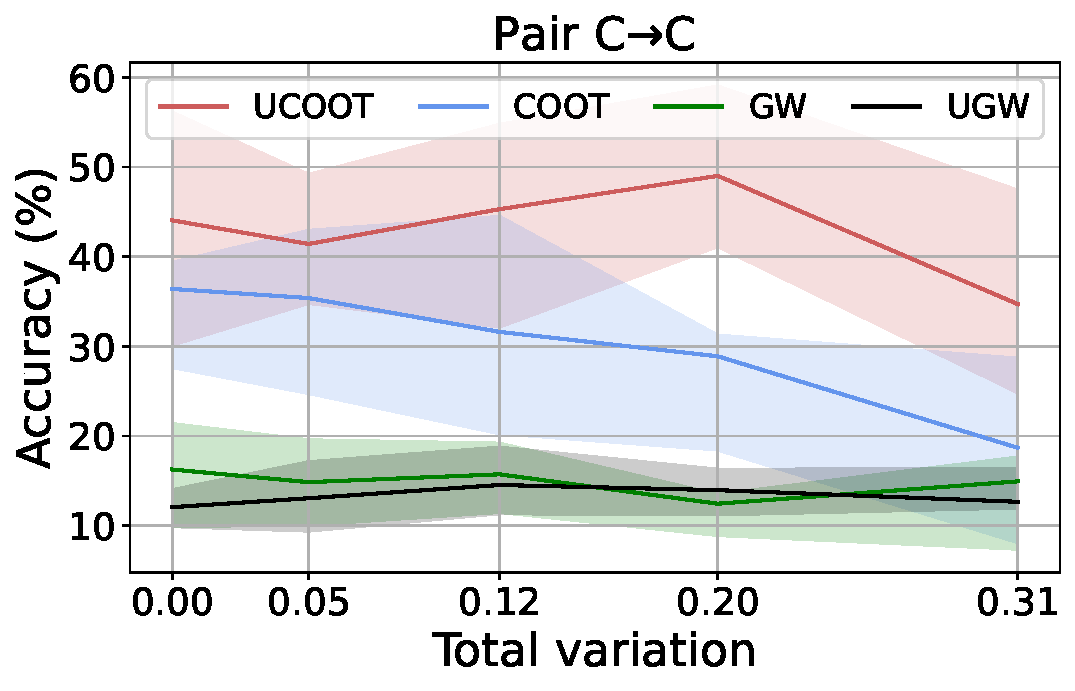
\includegraphics[width=\linewidth]{./Chapitre3/fig/summary_C_C.pdf}
  \vspace*{-7mm}
  \caption{Robustness to class proportion change for increasing TV on the class marginals.
  \label{f:hda_prop}}
\end{wrapfigure}
More precisely, we simulate a change in proportion only in the source domain
by selecting $20p$ samples per class for 4 amongst 10 classes with $p$
decreasing from $p=1$ to $p=0.2$. In this configuration,
the classes in the source domain are imbalanced and the unlabeled HDA problem becomes more difficult.
We report the performance of all the methods as a function of the Total Variation (TV)
between the class marginal distributions on one pair of datasets in \Cref{f:hda_prop}.
We can see that UCOOT is quite robust to change in class proportions,
while COOT experiences a sharp decrease in accuracy when the class distributions
become more imbalanced.

% We observe that in general, UCOOT is less stable than COOT, due to the mass
% relaxation nature. This is advantageous in the unsupervised HDA tasks, where, in absence of
% target labels, this relaxation provides flexibility to deals with the uncertainty of labels.
% For this reason, UCOOT usually outperforms COOT by large margins.
%
%\paragraph{Robustness to target shift}
%%%%%%%%%%%%%%%%%%%%%%%%%%%%%%%%%%%%%%%%%%%%
\subsubsection{Single-cell multi-omics alignment}

Finally, we present a real-world application of UCOOT for the alignment of single-cell measurements.
Recent advances in single-cell sequencing technologies allow biologists to measure
a variety of cellular features at the single-cell resolution, such as expression levels of genes
and epigenomic changes in the genome \citep{Buenrostro15,Chen19},
or the abundance of surface proteins \citep{CITEseq}. These multiple measurements produce
single-cell multi-omics datasets. These datasets measuring different biological phenomena
at the single-cell resolution allow scientists to study how the cellular processes are regulated,
leading to finer cell variations during development and diseases. However, it is hard to obtain
multiple types of measurements from the same individual cells due to experimental limitations.
Therefore, many single-cell multi-omics datasets have disparate measurements from different
sets of cells. As a result, computational methods are required to align the cells and
the features of the different measurements to learn the relationships between them that help
with data analysis and integration. Multiple tools \citep{Pamona, Seurat, Liu2019},
including GW \citep{Pamona, Demetci22} and UGW \citep{Demetci22-2} based methods,
have shown good performance for cell-to-cell alignments.
% However,  aligning both samples and features is a more challenging and critical task for this domain that can be solved by the UCOOT formulation.
However, aligning both samples and features is a more challenging and critical task that
GW and UGW-based methods cannot address
%\pinar{since they compute alignments between intra-domain distances, discarding features \citep{Demetci22, Pamona, Demetci22-2}}.
Here we provide an application of UCOOT to simultaneously align the samples and features
in a single-cell multi-omics dataset.
%
%how the features in different molecular features relate to one another.
%As a result, we require computational methods to align the cells and the features of the different measurements to obtain correspondence between similar cells and features. This correspondence information can help investigate which features in one domain (e.g., genes) match the ones (e.g., proteins) in the other domain.
%

\begin{figure}[t]
    \centering
    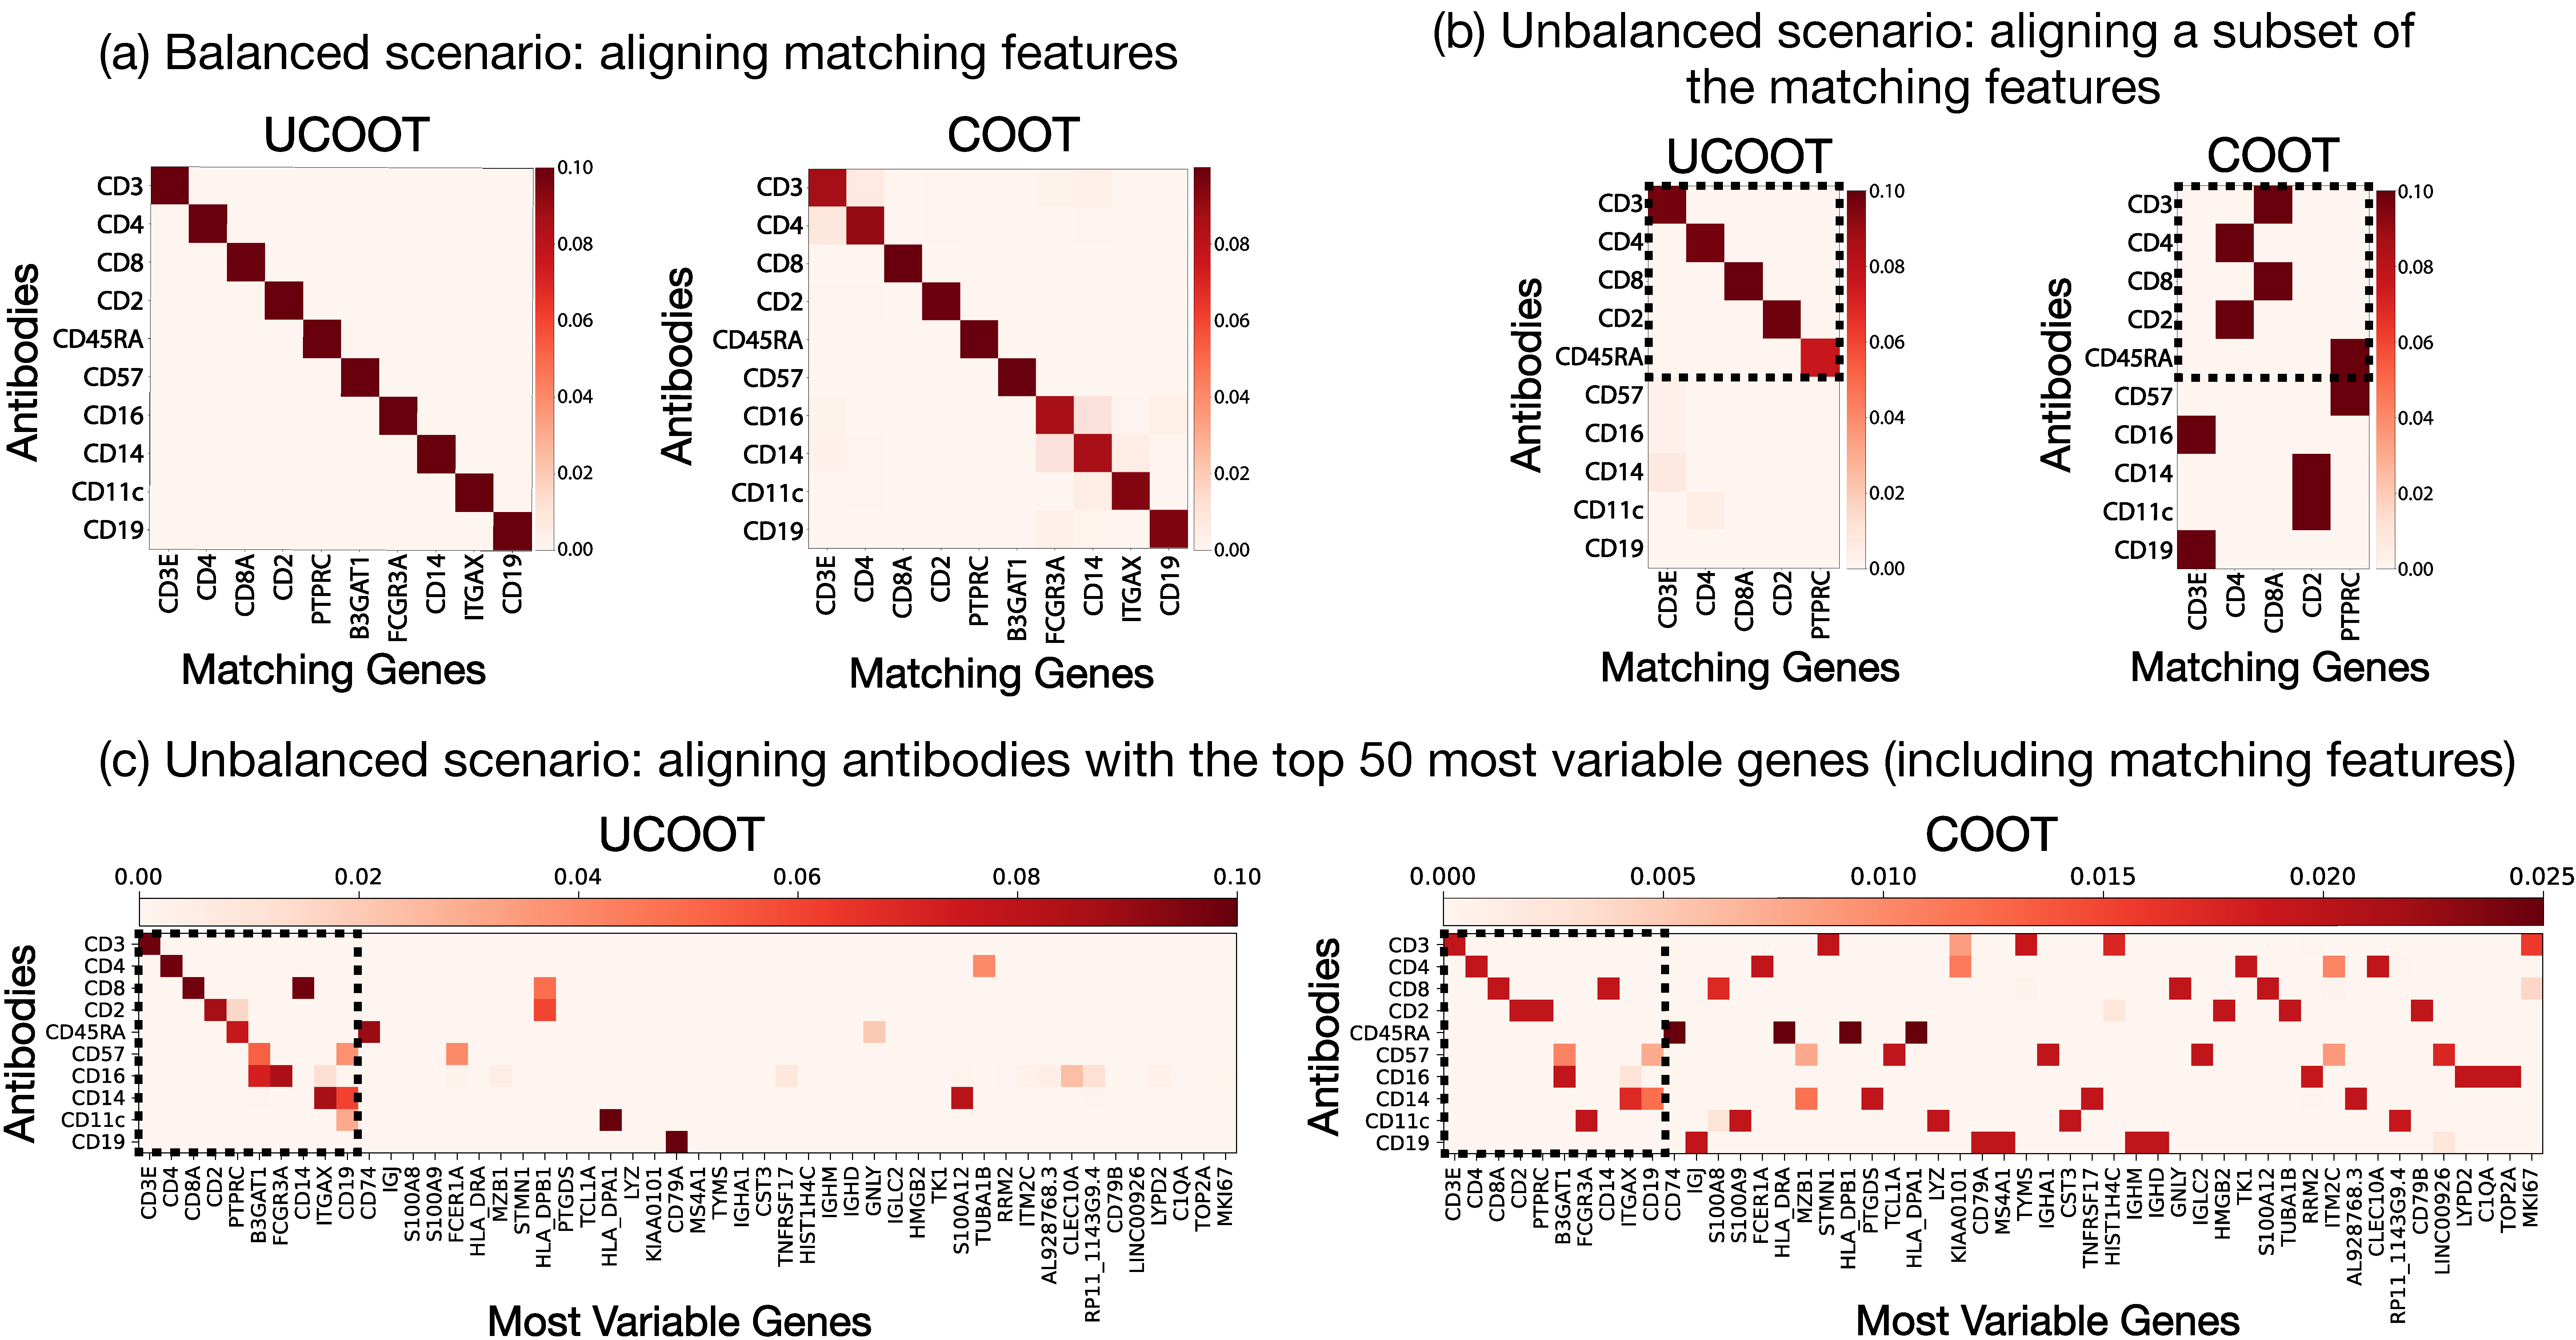
\includegraphics[trim={0.2cm 0.2cm 0.8cm 0.5cm}, clip, width=\linewidth, keepaspectratio=true]{./Chapitre3/fig/genes-alignments.pdf}
    \caption{Feature alignments on the single-cell multi-omics dataset of COOT and UCOOT between antibodies (surface proteins) and their matching genes (that encode them). \textbf{(a)} The features are sorted such that the correct alignment would yield a diagonal matrix. \textbf{(b)} Only five of the correct gene matches are kept (the last five genes from (a) are excluded). \textbf{(c)} Alignments between the ten antibodies and the top 50 most variable genes, including the matching genes.
    For \textbf{(b)} and \textbf{(c)}, the diagonal within the dashed square highlights the correct matches.
    Overall, UCOOT gives better feature alignments.
    \label{fig:multiomics}}
\end{figure}

\paragraph{Dataset} For demonstration, we choose a dataset generated by
the CITE-seq experiment \citep{CITEseq},
which simultaneously measures gene expression and antibody (or surface protein)
abundance in single cells. From this dataset, we use 1000 human peripheral blood cells,
which have ten antibodies and 17,014 genes profiled. We selected this specific dataset
as we know the ground-truth correspondences on both the samples (\ie, cells)
and the features (\ie, genes and their encoded antibodies), thus allowing us to quantify
and compare the alignment performance of UCOOT and COOT.
As done previously \citep{Pamona, Demetci22, Liu2019}, we quantify the cell alignment performance
by calculating the fraction of cells closer than the true match (FOSCTTM) of each cell
in the dataset and averaging it across all cells. This metric quantifies alignment error,
so lower values are more desirable. The feature alignments are measured by calculating
the accuracy of correct matching.

% \paragraph{Data Preprocessing} \label{CITEseq_exp_appendix}
% For the single-cell multi-omics experiments, we use the ``PBMC'' dataset from Stoeckius
% \textit{et al} \citep{CITEseq}, accessed on Gene Expression Omnibus (GEO) with the
% accession code: \href{https://www.ncbi.nlm.nih.gov/geo/query/acc.cgi?acc=GSE100866}{GSE100866}.
% This dataset contains a mix of 7,985 mouse and human peripheral blood mononuclear cells (PBMC)
% and profiles ten antibodies, 17,014 human genes, and 12,915 mouse genes. To pick the human cells,
% we follow the description in \citep{CITEseq}, and select the cells that have at least 500,
% and more than 90\% of all unique molecular identifiers (UMIs) mapped to the human genes
% (rather than the mouse genes). From the resulting $\sim 4500$ cells, we pick the first 1000
% to use in our experiments. We use the CLR-normalized antibody count data provided in GEO
% and apply log normalization to the gene expression data using Seurat package in R to
% remove biases in sequencing across cells \citep{Seurat}. Prior to alignment,
% we follow the existing single-cell alignment methods \citep{Demetci22, Demetci22-2,Liu2019,singh20},
% and also apply L2 normalization to both modalities. The top 50 most variable genes
% (\Cref{fig:multiomics}(c)) are selected using the \texttt{FindVariableFeatures()}
% function from \citep{Seurat}.

\paragraph{Hyperparameter tuning} Hyperparameters were tuned using grid search.
For both COOT and UCOOT, we considered the following range for the entropic regularization
coefficients $\varepsilon_f, \varepsilon_s \in \{1e-5, 5e-5, 1e-5, 5e-4, ... ,0.1, 0.5\}$.
For the mass relaxation coefficients $\rho_1, \rho_2 $ in UCOOT, the following range
was considered $\rho_1, \rho_2 \in \{1e-3, 5e-3, 0.01, 0.05, 0.1, 0.5, 1, 5, 10, 50 ,100\}$.
Each combination of hyperparameters were run on three randomly chosen subsets of the dataset
that included 30\% of the samples and the hyperparameter combinations that on average yielded
the highest feature matches and lowest FOSCTTM were picked for the experiments on the full dataset.

% I'll move the details about the original dataset to the Appendix
% The particular dataset we work with profiles a mix of 7,985 human and mouse peripheral blood mononuclear cells and contains measurements on 10 antibodies, 17014 human genes and 12915 mouse genes. We select 1000 human cells from this dataset to work with.

\paragraph{Results in balanced scenarios} First, we select and align the same number of samples and features
across the two datasets. For this, we subset the gene expression domain with the ten genes that
match to the ten antibodies they express. Original data contains the same number of cells
across domains since both domains are simultaneously measured in the same single-cells.
We observe that both UCOOT and COOT can correctly align features (\Cref{fig:multiomics}~(a))
and the cells across the two measurements. However,
UCOOT gives better performance, as demonstrated by a lower FOCSTTM score (0.0062 vs 0.0127)
for cells. Both COOT and UCOOT recover the diagonal for matching features (100\% accuracy),
but UCOOT recovers the exact matching, likely due to its robustness to noise,
whereas COOT assigns weights to other features as well.

\paragraph{Results in unbalanced scenarios} Next, we perform alignment with an unequal number of features.
This setting is more likely to occur for real-world single-cell datasets as different features
are measured. In the first simple scenario, we align the ten antibodies with only a subset (five)
of their matching genes. As visualized in \Cref{fig:multiomics}~(b),
COOT struggles to find the correct feature alignments (60\% accuracy),
which would lie in the diagonal of the highlighted square (dashed lines). However,
the relaxation of the mass conservation constraint in UCOOT allows it to shrink
the mass of antibodies that lack matches in the gene expression domain,
leading do higher accuracy (100\% accuracy).

Next, we align the ten antibodies with
the 50 most variable genes in the dataset, including their matching genes.
This alignment task is the most realistic scenario, as single-cell multi-omics data
consists of high-dimensional datasets with a different number of features for different measurements.
% \pinar{Moreover, many of these genes show consistent expression levels across }
Therefore, biologists focus their analyses on the reduced set of most variable features (e.g. genes).
It is also the most computationally challenging case among all our experiments on this dataset.
Hence, we provide sample-level supervision to both methods by giving a cost penalization matrix
based on the correct sample alignments to the sample alignment computation.
We see in \Cref{fig:multiomics}(c) that in comparison to COOT (50\% accuracy),
UCOOT recovers more of the correct feature alignments (70\% accuracy),
and yields fewer redundant alignments.
Note that UCOOT avoids incorrect mappings by locally shrinking the mass of the features or samples
that lack correspondences. This avoids subsequent incorrect downstream analysis of
the integration results. This property can also help users to discover rare cell types
by observing the extent of mass relaxation per cell or prune uninformative features in
the single-cell datasets.

%Similarly to the alignment in \Cref{fig:multiomics}(b), this is thanks to the mass shrinkage of the features that lack correspondences. By locally adjusting the mass in transport, UCOOT tends to avoid assigning correspondences to samples or features that lack matches across the aligned domains. With this, UCOOT can help users to detect outliers that can result from experimental artifacts,
%(such as rare cell types or lowly expressed genes that are not captured well by a sequencing technology), prune features or discover rare cell types.}

Lastly, we also consider the case of unequal number of samples across the two measurements.
This case is common in real world single-cell multi-omics datasets that are not
simultaneously measured. \citet{Demetci22-2} have shown that
single-cell alignment methods that do not account for this mismatch yield poor alignment results.
Therefore, we downsample the number of cells in one of the domains by 25\%
and perform alignment with the full set of cells in the other domain.
We compute the FOSCTTM score for all cells that have a true match in the dataset and
report the average values. UCOOT continues to yield a low FOSCTTM score (0.0081 compared to 0.0062
in the balanced scenario), while COOT shows a larger drop in performance
(0.1342 compared to 0.0127 in the balanced scenario).

\subsection{Discussion and conclusion}
\label{sec:conclusion}

In this work, we present an extension of COOT called unbalanced COOT,
where the hard constraint on the marginal distributions is replaced by a soft control via
the KL divergence. The resulting problem not only benefits from the flexibility of COOT
but also enjoys the provable robustness property under the presence of outliers,
which is not the case for COOT. The experimental results confirm our findings,
yielding a very competitive performance in the unsupervised HDA task, as well as
meaningful feature couplings for the single-cell multi-omics alignment. Also,
while UCOOT introduces additional hyper-parameters, domain knowledge can help narrow down
the range of feasible values, thus reducing the time and computational cost of the tuning process.
Further investigation should be carried out to fully understand and assess
the observed efficiency of UCOOT in real-world applications,
and also explore the possibilities of UCOOT in more diverse applicative settings,
including its use as a loss in deep learning architectures.
Lastly, from a theoretical perspective, statistical properties such as
sample complexity or stability analysis are needed to better understand
the intricate relations between the two sample and feature couplings.
%Future works may also focus on justifying how the relaxation of marginal constraints allows to cope with the class imbalance and provides empirically better initialization to the approximation scheme of COOT, as observed in the experiments. Last but not least, it is interesting to study the connection with the unbalanced GW distance, since in practice, it is estimated using its lower bound, which is in fact a special of UCOOT.

% The last section presents the results from \citep{Thual22} and addresses the applications of
% unbalanced extension of fused Gromov-Wasserstein in human brains alignments.
% Individual brains vary in both anatomy and functional organization, even within a given species.
% Inter-individual variability is a major impediment when trying to draw generalizable conclusions
% from neuroimaging data collected on groups of subjects.
% Current co-registration procedures rely on limited data, and thus lead to very coarse
% inter-subject alignments.
% In this work, we present a novel method for inter-subject alignment based on Optimal Transport,
% denoted as Fused Unbalanced Gromov-Wasserstein (FUGW).
% The method aligns cortical surfaces based on the similarity of their functional signatures in
% response to a variety of stimulation settings, while penalizing large deformations of
% individual topographic organization.
% We demonstrate that FUGW is well-suited for whole-brain landmark-free alignment.
% The unbalanced feature allows to deal with the fact that functional areas
% vary in size across subjects. Our results show that FUGW alignment significantly
% increases between-subject correlation of activity for independent functional data,
% and leads to more precise mapping at the group level.

% 
%%%%%%%%%%%%%%%%%%%%%%%%%%%%%%%%%%%%%%%%%%%%%%
\section{Inexact Bregman Proximal Point for Entropic Unbalanced Optimal Transport}
\label{sec:input}

This section is an ongoing work on an alternative solver for the entropic UOT problem
\ref{eq:discrete_ent_uot}, which has not yet been studied in the literature,
to the best of our knowledge.
We called this approach \textit{INexact Proximal Unbalanced optimal Transport} (INPUT),
since it is a straightforward application of the inexact Bregman Proximal Point (BPP) algorithm
to the UOT problem. We present the derivation of INPUT, then illustrate how
it can overcome the limitations of the MM and Sinkhorn-based methods,
while being orders of magnitude faster in our toy experiments. Despite the simplicity,
its convergence analysis remains a challenging open problem and is under our active research.

\subsection{Motivation, optimization and algorithm}

While the Bregman Proximal Point method \citep{Chen93} applies to the class of Bregman divergences,
we will exclusively focus on the KL divergence throughout this thesis.
\begin{definition}
  Given a nonepmpty closed convex set of $E \subset \bbR^d_{\geq 0}$
  and a proper closed convex function $f: E \to \bbR$, consider the following
  convex optimization problem
  \begin{align}
    \min_{x \in E} f(x).
  \end{align}
  For learning rate $\eta > 0$, the exact BPP scheme with respect to the KL divergence reads
  \begin{align}
    \label{eq:bppa}
    x^{(t+1)} = \argmin_{x \in E} f(x) + \eta \kl(x, x^{(t)}),
  \end{align}
  and the inexact BPP scheme reads
  \begin{align}
    \label{eq:bppa_inexact}
    x^{(t+1)} \approx \argmin_{x \in E} f(x) + \eta \kl(x, x^{(t)}).
  \end{align}
  Here, $x^{(t+1)}$ is only an approximate solution in some predefined sense.
\end{definition}
When applying to Problem \eqref{eq:discrete_ent_uot}, the exact BPP iteration boils down to solving
\begin{align}
\label{eq:bpp_uot}
  &P^{(t+1)} \\
  &= \argmin_{P \in \bbR^{m \times n}_{\geq 0}}
  \langle C, P \rangle + \rho_1 \kl(P_{\# 1} | \mu)
  + \rho_2 \kl(P_{\# 2} | \nu) + \varepsilon \kl(P | \gamma) + \eta \kl(P | P^{(t)}) \\
  &= \argmin_{P \in \bbR^{m \times n}_{\geq 0}}
  \left \langle C - \eta \log \frac{P^{(t)}}{\gamma}, P \right \rangle
  + \rho_1 \kl(P_{\# 1} | \mu) + \rho_2 \kl(P_{\# 2} | \nu) + (\varepsilon + \eta) \kl(P | \gamma).
\end{align}
This is nothing but an entropic UOT problem with modified cost and regularization.
Thus, any solvers discussed in \Cref{sub:uot_optim} can be used. In particular,
by construction, BPP is naturally applicable to the unregularized UOT.
In practice, the exact BPP may not be an efficient algorithm to solve the UOT problem since
it requires solving \textbf{exactly} many entropic subproblems. This can be computationally expensive,
especially when the learning rate is small.

While the inexact BPP scheme has recently been applied to the balanced OT \citep{Xie20,Yang22},
we are not aware of any extension to the unbalanced counterpart.
Our proposed method follows directly from \citep{Xie20}, which is simple to implement and
usually performs well in practice. In particular,
we only require running a few Sinkhorn iterations for each entropic subproblem and
use the approximated coupling as input for the next BPP iteration.
The algorithmic details of INPUT can be found in \Cref{alg:isppa}.
\begin{algorithm}[t]
  \caption{INPUT algorithm for Problem \eqref{eq:discrete_ent_uot}.}
  \label{alg:isppa}
\begin{algorithmic}[1]
  \STATE \textbf{Input:} cost matrix $C \in \bbR^{m \times n}$,
  measures $\mu \in \bbR^m_{> 0}, \nu \in \bbR^n_{> 0}, \gamma \in \bbR^{m \times n}_{> 0}$,
  regularization $\varepsilon \geq 0$, relaxation parameters $\rho_1, \rho_2 > 0$,
  learning rate $\eta > 0$.
  \FOR{$t=1, \dots, T$}
  \STATE Calculate new cost: $C^{(t+1)} \gets C - \eta \log \Big( \frac{P^{(t)}}{\gamma} \Big)$.
  \STATE Solve approximatively the entropic UOT problem
  \begin{align}
    P^{(t+1)} \approx \argmin_{P \geq 0} \; \langle C^{(t+1)}, P \rangle +
    \rho_1 \kl(P_{\# 1} | \mu) + \rho_2 \kl(P_{\# 2} | \nu) + (\varepsilon + \eta) \kl(P | \gamma).
  \end{align}
  \ENDFOR
  \STATE \textbf{Output:} transport plan $P^{(T)}$.
\end{algorithmic}
\end{algorithm}

\subsection{Convergence analysis in the exact setting}

Let us start with the convergence analysis in case of exact BPP iteration \ref{eq:bpp_uot}.
Thanks to Lemma 3.3 and Theorem 3.4 in \citep{Chen93}, if $P^*$ is a minimizer of
Problem \eqref{eq:discrete_ent_uot}, then
\begin{enumerate}
  \item The sequence $\big( \kl(P^*, P^{(t)}) \big)_t$ is nonincreasing and converges to $0$.
  \item The sequence $\big( F(P^{(t)}) \big)_t$ is nonincreasing and
  \begin{align}
    \label{eq:chen_teboulle}
    F(P^{(t)}) - F(P^*) \leq \frac{\eta}{t} \kl(P^* | P^{(0)}).
  \end{align}
\end{enumerate}
The upper bound \eqref{eq:chen_teboulle} can be improved by further exploiting the property of
the objective function of Problem \eqref{eq:discrete_ent_uot}.
First, we introduce the notions of relative smoothness \citep{Bauschke17} and
strong convexity \citep{Lu18} of a function with respect to the KL divergence.
\begin{definition}
  \label{def:smooth-convex}
  Let $f:C \to \bbR$ be a differentiable convex function.
  Given $L \geq 0$, we say that $f$ is $L-$smooth relative to the KL divergence
  if for any $x, y \in C$,
  \begin{align}
    f(x) \leq f(y) + \langle \nabla f(y), x - y \rangle + L \; \kl(x, y).
  \end{align}
  Given $l \geq 0$, we say $f$ is $l-$strongly convex relative to the KL divergence
  if for any $x, y \in C$,
  \begin{align}
    f(x) \geq f(y) + \langle \nabla f(y), x - y \rangle + l\; \kl(x, y).
  \end{align}
\end{definition}

\begin{lemma}
  \label{lemma:convex-smoothness}
  $F$ is $\varepsilon$-strongly convex and $(\lambda_1 + \lambda_2 + \varepsilon)$-relatively smooth
  with respect to the KL divergence.
\end{lemma}
The following result is a simple generalization of Theorem 3.1 in \citep{Lu18}.
\begin{proposition}[Convergence rate of exact BPP for Problem \eqref{eq:discrete_ent_uot}]
  \label{prop:convergence-exact-sppa}
  For every $\eta > 0$, exact BPP scheme decreases the value of $F(\cdot)$ with each iteration $t$:
  the sequence $\big( F(\pi^{(t)}) \big)_t$ is monotonically decreasing.
  Moreover, if $\varepsilon \leq \eta \leq \lambda_1 + \lambda_2 + \varepsilon$,
  then we have
  \begin{align}
    F(\pi^{(t)}) - F(\pi^*)
    \leq \frac{\varepsilon}{\left( 1 +
    \frac{\varepsilon (\lambda_1 + \lambda_2 + \varepsilon)}{\eta (\lambda_1 + \lambda_2)} \right)^t - 1}
    \kl(\pi^* | \pi^{(0)}).
  \end{align}
\end{proposition}
It is not difficult to check that this bound is weaker than the one in
Inequality (\ref{eq:chen_teboulle}). Indeed,
\begin{align}
  \frac{\varepsilon}{\left( 1 +
  \frac{\varepsilon (\lambda_1 + \lambda_2 + \varepsilon)}{\eta (\lambda_1 + \lambda_2)} \right)^t - 1}
  \leq \frac{\varepsilon}{\frac{t \varepsilon(\lambda_1 + \lambda_2 + \varepsilon)}{\eta (\lambda_1 + \lambda_2)}}
  = \frac{\eta}{t} \frac{\lambda_1 + \lambda_2}{\lambda_1 + \lambda_2 + \varepsilon}
  \leq \frac{\eta}{t}.
\end{align}

\subsection{Convergence analysis in the inexact setting}

Despite the simplicity, it is difficult to analyze the convergence of INPUT.
In particular, while it is an immediate extension of the work of \citet{Xie20} on the balanced OT,
their proof techniques of the convergence can not be adapted to the unbalanced setting.
This is because they rely on the property of the set of admissible couplings,
which is not available in the UOT. Moreover, their assumptions and conditions are also
not trivial to verify in practice, thus the convergence results are mostly of theoretical interest.

The convergence analysis of the inexact BPP has already been studied at the same time
as the exact one. Typically, one can control the approximation error using
$\varepsilon$-subdifferential \citep{Burachik97,Kiwiel97},
or bounded subgradient \citep{Eckstein98,Rockafellar76}, to name a few.
We are studying the literature in this domain to identify the relevant criteria, which are
amenable to study the convergence and to verify in practice.

\subsection{Illustration on toy example}

\paragraph{Experimental setup}
We consider a synthetic dataset:
the source data $X$ contains $200$ points forming an ellipse and a square,
assigned with the same uniform probability on both shapes
$\mu = \frac{1}{200} \sum_{i=1}^{200} \delta_{x_i}$. The target data $Y$ also contains $200$ points
forming an ellipse and a circle, assigned with the histogram
$\nu = \frac{3}{200} \sum_{j=1}^{30} \delta_{y_j \in \text{Circle}} +
\frac{7}{200} \sum_{j=31}^{100} \delta_{y_j \in \text{Circle}} +
\frac{7}{200} \sum_{j=1}^{100} \delta_{y_j \in \text{Ellipse}}$.
The objective in this experiment is to estimate the entropic UOT cost, where
we choose $\gamma = \mu \otimes \nu$ and the cost $C(x, y) = || x - y||^2_2$.

\paragraph{Competing methods}
For INPUT, we consider $3$ versions corresponding to $3$ solvers for the inner entropic UOT problem:
\texttt{INPUT-Sinkhorn}, \texttt{INPUT-TI-v2}, \texttt{INPUT-MM}.
Here, we choose the variant of Sinkhorn-TI (\Cref{alg:TI_Sinkhorn_variant})
since it is more simple to implement, yet appears to perform comparably to the Sinkhorn-TI.
The Sinkhorn-based methods include
\texttt{Sinkhorn} (\Cref{alg:Sinkhorn_algo}), \texttt{Sinkhorn-TI-v1} (\Cref{alg:TI_Sinkhorn})
and its variant \texttt{Sinkhorn-TI-v2} (\Cref{alg:TI_Sinkhorn_variant}).
We emphasize that all Sinkhorn-based methods require log-domain implementation
for numerical stability, whereas INPUT does not suffer this issue,
thus is implemented with direct vector-matrix multiplication.
Apart from these $2$ families of solvers, we also evaluate the performance of
Majorization-Minimization algorithm \texttt{MM}.

\paragraph{Results}
We set up $4$ scenarios to verify if INPUT can overcome the limitations of other existing methods.
More precisely, the first one considers the situation of small relaxations and large regularization.
It is an easy test and we expect that all methods perform well.
In the second one, we fix the relaxations but choose small regularization
in order to hinder convergence of Sinkhorn-based methods.
The third scenario uses fixed regularization but very large marginal relaxations to slow down
the convergence of MM.
The last one combines small regularization and very large relaxations. It is designed to challenge
both Sinkhorn and MM methods.

It is clear that the INPUT family consistently and significantly outperforms other solvers,
The distinction becomes even more visible in the regimes where Sinkhorn and MM struggle.
Except for the first scenario, by contrast to its competitors,
it seems that INPUT does not require compensating the running time for the quality of the estimation.
We also observe that, within the family of INPUT,
combining INPUT with Sinkhorn-TI yields the most efficient algorithm.
Amongst the Sinkhorn-based solvers, Sinkhorn-TI shows clear improvement over Sinkhorn,
even though this advantage quickly diminishes when regularization is small.

\begin{table}[]
  \small
  \centering
  \begin{tabular}{|cc|c|c|c|c|}
  \hline
  \multicolumn{2}{|c|}{} &
    \textbf{\begin{tabular}[c]{@{}c@{}}Scenario 1\\ $\rho_1 = 40$\\ $\rho_2 = 50$\\ $\varepsilon = 1$\end{tabular}} &
    \textbf{\begin{tabular}[c]{@{}c@{}}Scenario 2\\ $\rho_1 = 40$\\ $\rho_2 = 50$\\ $\varepsilon = 1e-3$\end{tabular}} &
    \textbf{\begin{tabular}[c]{@{}c@{}}Scenario 3\\ $\rho_1 = 4000$\\ $\rho_2 = 5000$\\ $\varepsilon = 1$\end{tabular}} &
    \textbf{\begin{tabular}[c]{@{}c@{}}Scenario 4\\ $\rho_1 = 4000$\\ $\rho_2 = 5000$\\ $\varepsilon = 1e-3$\end{tabular}} \\ \hline
  \multicolumn{1}{|c|}{\multirow{3}{*}{\textbf{\begin{tabular}[c]{@{}c@{}}Sinkhorn\\ family\end{tabular}}}} &
    \textbf{Sinkhorn} &
    \begin{tabular}[c]{@{}c@{}}0.275 $\pm$ 0.011\\ {\color{blue}{{41.618}}} \end{tabular} &
    \begin{tabular}[c]{@{}c@{}}55.946 $\pm$ 5.893\\ 40.588\end{tabular} &
    \begin{tabular}[c]{@{}c@{}}{\color{red}{{0.020 $\pm$ 0.002}}} \\ 57.667\end{tabular} &
    \begin{tabular}[c]{@{}c@{}}No convergence at \\ this tolerance\end{tabular} \\ \cline{2-6}
  \multicolumn{1}{|c|}{} &
    \textbf{TI-v1} &
    \begin{tabular}[c]{@{}c@{}}0.389 $\pm$ 0.018\\ {\color{blue}{{41.618}}}\end{tabular} &
    \begin{tabular}[c]{@{}c@{}}37.679 $\pm$ 0.926\\ {\color{red}{{40.576}}}\end{tabular} &
    \begin{tabular}[c]{@{}c@{}}1.118 $\pm$ 0.047\\ 57.613\end{tabular} &
    \begin{tabular}[c]{@{}c@{}}31.088 $\pm$ 0.505\\ 56.834\end{tabular} \\ \cline{2-6}
  \multicolumn{1}{|c|}{} &
    \textbf{TI-v2} &
    \begin{tabular}[c]{@{}c@{}}0.318 $\pm$ 0.013\\ {\color{blue}{{41.618}}}\end{tabular} &
    \begin{tabular}[c]{@{}c@{}}31.679 $\pm$ 2.919\\ {\color{red}{{40.576}}}\end{tabular} &
    \begin{tabular}[c]{@{}c@{}}0.871 $\pm$ 0.034\\ 57.613\end{tabular} &
    \begin{tabular}[c]{@{}c@{}}24.828 $\pm$ 0.243\\ 56.834\end{tabular} \\ \hline
  \multicolumn{1}{|c|}{\multirow{3}{*}{\textbf{\begin{tabular}[c]{@{}c@{}}INPUT\\ family\end{tabular}}}} &
    \textbf{Sinkhorn} &
    \begin{tabular}[c]{@{}c@{}}0.190 $\pm$ 0.008\\ {\color{blue}{{41.618}}}\end{tabular} &
    \begin{tabular}[c]{@{}c@{}}0.676 $\pm$ 0.032\\ {\color{blue}{{40.521}}}\end{tabular} &
    \begin{tabular}[c]{@{}c@{}}1.143 $\pm$ 0.048\\ {\color{blue}{{57.608}}}\end{tabular} &
    \begin{tabular}[c]{@{}c@{}}1.387 $\pm$ 0.026\\ {\color{blue}{{55.866}}}\end{tabular} \\ \cline{2-6}
  \multicolumn{1}{|c|}{} &
    \textbf{TI-v2} &
    \begin{tabular}[c]{@{}c@{}}{\color{red}{{0.149 $\pm$ 0.008}}}\\ {\color{blue}{{41.618}}} \end{tabular} &
    \begin{tabular}[c]{@{}c@{}}{\color{red}{{0.649 $\pm$ 0.013}}}\\ {\color{blue}{{40.521}}} \end{tabular} &
    \begin{tabular}[c]{@{}c@{}}{\color{blue}{{0.018 $\pm$ 0.002}}} \\ {\color{red}{{57.609}}}\end{tabular} &
    \begin{tabular}[c]{@{}c@{}}{\color{blue}{{0.079 $\pm$ 0.010}}} \\ {\color{red}{{55.868}}}\end{tabular} \\ \cline{2-6}
  \multicolumn{1}{|c|}{} &
    \textbf{MM} &
    \begin{tabular}[c]{@{}c@{}} {\color{blue}{{0.068 $\pm$ 0.006}}} \\ 41.627\end{tabular} &
    \begin{tabular}[c]{@{}c@{}} {\color{blue}{{0.186 $\pm$ 0.007}}} \\ 40.640\end{tabular} &
    \begin{tabular}[c]{@{}c@{}}1.038 $\pm$ 0.026\\ 57.738\end{tabular} &
    \begin{tabular}[c]{@{}c@{}}1.028 $\pm$ 0.021\\ 56.723\end{tabular} \\ \hline
  \multicolumn{2}{|c|}{\textbf{MM}} &
    \begin{tabular}[c]{@{}c@{}}0.193 $\pm$ 0.010\\ {\color{red}{{41.621}}} \end{tabular} &
    \begin{tabular}[c]{@{}c@{}}0.864 $\pm$ 0.024\\ 40.558\end{tabular} &
    \begin{tabular}[c]{@{}c@{}}0.726 $\pm$ 0.046\\ 59.089\end{tabular} &
    \begin{tabular}[c]{@{}c@{}}{\color{red}{{0.944 $\pm$ 0.026}}} \\ 57.829\end{tabular} \\ \hline
  \end{tabular}
  \caption{Time $\pm$ standard deviation (in seconds) required to reach the predefined tolerance
  (first line) and entropic UOT cost (second line). The lower score the better.
  {\color{blue}{{Blue number}}} indicates the best score.
  {\color{red}{{Red number}}} indicates the second best score.
  \label{t:uot_time_compare}}
\end{table}

\subsection{Discussion}

While this experiment is mainly for the proof-of-concept purpose,
it shows that INPUT is a promising alternative solver for the UOT problem.

\paragraph{Strengths of INPUT}
INPUT has two very appealing features. First, it overcomes the limitations of
the MM and Sinkhorn-based algorithms. In particular,
it can, not only handle both balanced/unbalanced, and unregularized/regularized settings,
but also, empirically, can converge very fast to the optimal plan and the global minimum,
even in the regimes of very small regularization (where Sinkhorn-based methods struggles),
or of very large relaxation (where MM wrestles).
We summarize the applicability of these algorithms in \Cref{t:uot_algo_compare}.

Second, the presence of learning rate $\eta$
increases the level of regularization in the inner entropic UOT subproblem,
thus brings two important benefits. The first one is on the reduction of number of iterations:
the larger the regularization, the faster the Sinkhorn algorithm converges. As a consequence,
running only a few iterations is usually enough to obtain a decent approximation of
the true solution. The second advantage is on the acceleration per BPP iteration. In practice,
when the regularization is not too small, one can ignore the log-domain implementation
and employ the one with direct vector-matrix multiplication,
without any concern about the numerical overflow issue.
As a result, this allows to speed up the calculation of the iterates.

\paragraph{Weaknesses of INPUT} There is no free lunch. INPUT has two drawbacks.
First, the cost matrix must be recalculated at the beginning of each BPP iteration.
This can be computationally expensive and prevents INPUT from being scalable.
Second, while tuning the learning rate is neither too tricky nor difficult,
it may take some effort to find an appropriate value. One possible workaround,
which usually works well in practice, is to start with $\eta$ small and not too far from $\varepsilon$.
The intuition of this heuristic comes from \Cref{prop:convergence-exact-sppa} of exact BPP scheme,
which indicates that, for fixed initialization, the smaller the learning rate, the smaller
the potential gap between the estimation and the minimum.
\begin{table}[t]
	\centering
		\begin{tabular}{|l|c|c|c|c|}
    \hline
    & \textbf{\makecell{Scaling}}
    & \textbf{\makecell{TI-Sinkhorn}} & \textbf{MM} & \textbf{INPUT} \\
    \hline
    \makecell[l]{Unregularized \\ setting} & \nomark & \nomark & \yesmark & \yesmark \\
    \hline
    \makecell[l]{Balanced \\ setting} & \yesmark & \yesmark & \nomark  & \yesmark  \\
    \hline
    \makecell[l]{Semi-relaxed \\ setting} & \yesmark & \yesmark & \nomark  & \yesmark  \\
    \hline
    \makecell[l]{Major \\ drawbacks} & \makecell{Very slow conv. \\ for small $\varepsilon$}
    & \makecell{Slow conv. \\ for small $\varepsilon$}
    & \makecell{Slow conv. \\ for large $\rho$}
    & \makecell{Cost recalculation, \\
    extra tuning of \\ hyperparameters} \\
    \hline
		\end{tabular}
		\caption{Summary of features of algorithms for entropic UOT problem \eqref{eq:discrete_ent_uot}.
    Unregularized setting refers to $\varepsilon = 0$, balanced setting corresponds to
    $\rho_1 = \rho_2 = \infty$ and semi-relaxed setting refers to either $\rho_1 = \infty$
    or $\rho_2 = \infty$.
    \label{t:uot_algo_compare}}
\end{table}

\paragraph{Can we adapt INPUT to solve the squared $l_2$-regularized Problem \eqref{uot_l2} ?}
In theory, yes, since the squared $l_2$-norm is a Bregman divergence,
thus the (inexact) BPP scheme is applicable. However, comparing to the MM solver,
we doubt that it would bring any gain in convergence speed. Indeed,
recall that the main motivation of INPUT comes from the poor convergence behavior of Sinkhorn
algorithm when \textbf{regularization} is small. For this reason, adding more regularization
to each BPP iteration helps accelerating the calculation
and improving the convergence of the algorithm. By contrast,
the case of squared $l_2$-norm does not suffer the same issue,
but rather on the \textbf{relaxation} parameters. So, more regularization does not help.
% \section{Fused Unbalanced Gromov-Wasserstein}

%%%%%%%%%%%%%%%%%%%%%%%%%%%
\subsection{Introduction}
\label{sec:introduction}

The availability of millimeter or sub-millimeter anatomical or functional brain images has opened
new horizons to
neuroscience, namely that of mapping cognition in the human brain and detecting markers of diseases.
%
Yet this endeavour has stumbled on the roadblock of inter-individual
variability: while the overall organization of the human brain is largely invariant,
two different brains (even from monozygotic twins \citep{pizzigali2020})
may differ at the scale of centimeters in shape, folding pattern, and functional responses.
%
% While variability is a hindrance to brain mapping,
The problem is further complicated by the fact that functional images
are noisy, due to imaging limitations and behavioral
differences across individuals that cannot be easily overcome.
%
The status quo of the field is thus to rely on anatomy-based inter-individual alignment
that approximately matches the outline of the brain \citep{ants}
as well as its large-scale cortical folding patterns \citep{fs_reconall,fischl_freesurfer_2012}.
%
Existing algorithms thus coarsely match anatomical features with diffeomorphic transformations,
by warping individual data to a simplified template brain.
Such methods lose much of the original individual detail and blur the functional information
that can be measured in brain regions (see \Cref{fig:intro}).

\begin{figure}[ht]
    \centering
    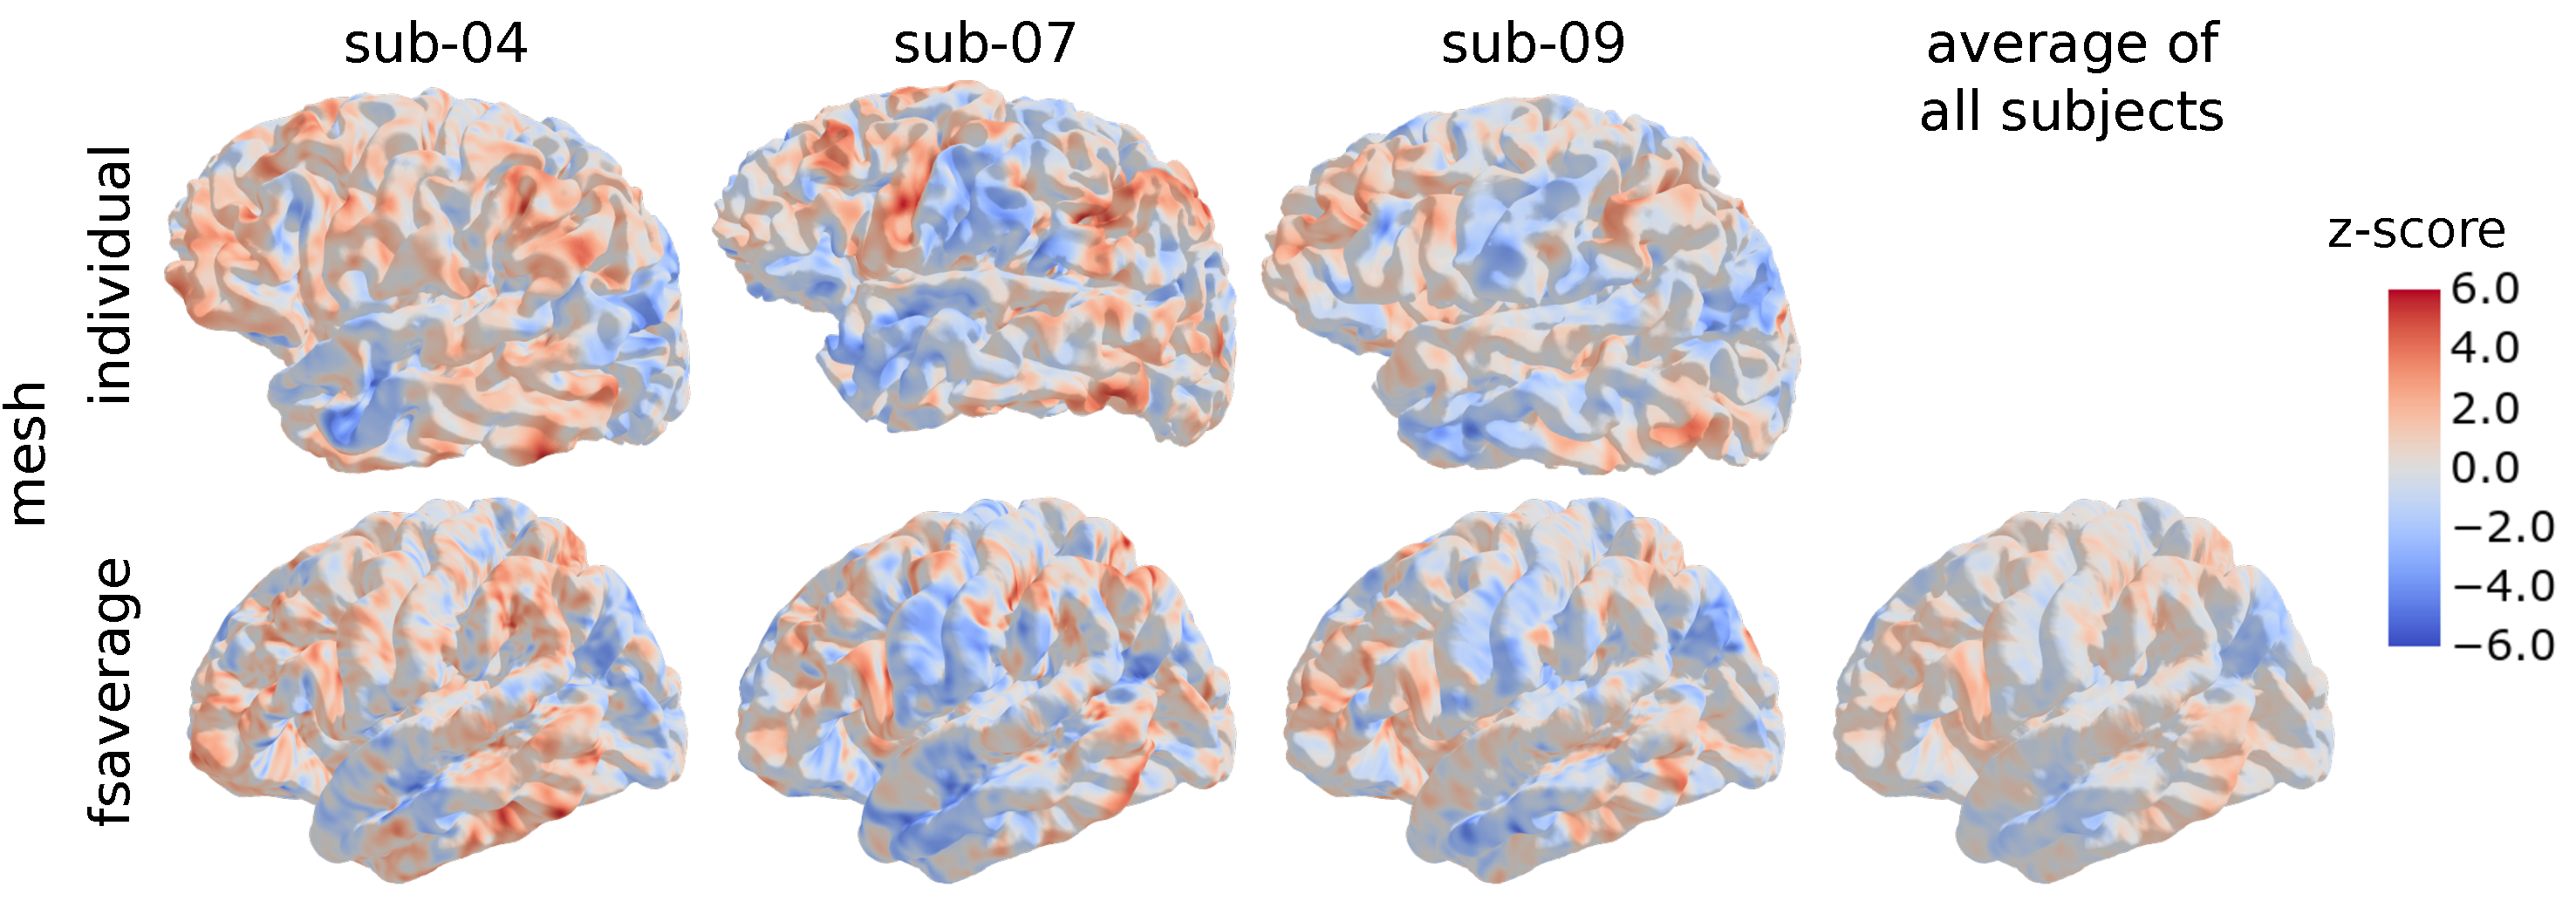
\includegraphics[width=\columnwidth]{./Chapitre4/figures/intro_variation.pdf}
    \caption{
        \textbf{High variability in human anatomies and functional MRI responses across subjects}
        In this experiment contrasting areas of the brain
        which respond to mathematical tasks against other that
        don't, we observe great variability in locations and strength of brain activations across subjects (row 1).
        The classical approach consists in wrapping this data
        to a common surface template (row 2), where they can be averaged, often resulting in
        loss of individual details and detection power.
        These images were generated using Nilearn software \citep{abraham_machine_2014}.
    }
    \label{fig:intro}
\end{figure}
In order to improve upon the current situation, a number of challenges have to be addressed:
%
\textit{(i)} There exists no template brain with functional information,
which by construction renders any cortical matching method blind to function.
This is unfortunate, since functional information is arguably the most accessible marker
to identify cortical regions and their boundaries \citep{Glasser2016-ha}.
%
\textit{(ii)} When comparing two brains -- coming from individuals or from a template --
it is unclear what regularity should be imposed on the matching \citep{vanessen2012}.
While it is traditional in medical imaging to impose diffeomorphicity \citep{ants},
such a constrain does not match the frequent observation that brain regions vary
across individuals in their fine-grained functional organization \citep{Glasser2016-ha,schneider2019}.
% \bt{find other ref}
%
\textit{(iii)} Beyond the problem of aligning human brains, it is an even greater challenge
to systematically compare functional brain organization in two different species,
such as humans and macaques \citep{neubert_comparison_2014,mars_whole_2018,xu_cross-species_2020,eichert_cross-species_2020,}.
Such inter-species comparisons intro9duce a more extreme form of variability in the correspondence model.

\paragraph{Related work}
%
Several attempts have been made to constrain the brain alignment process by using
functional information. The first one consists in introducing functional maps into
the diffeomorphic framework and search for a smooth transformation that matches
functional information \citep{sabuncu_function-based_2010,yeo_spherical_2010,robinson_msm_2014},
the most popular framework being arguably Multimodal Surface Matching (MSM)
\citep{robinson_msm_2014,Glasser2016-ha}.

A second family of less constrained functional alignment approaches have been proposed,
based on heuristics, by matching information in small, possibly overlapping,
cortical patches \citep{haxby_common_2011,Tavor2016-rl,bazeille_empirical_2021}.
%
This popular framework has been called \emph{hyperalignment}
\citep{haxby_common_2011,guntupalli_model_2016}, or \emph{shared response models} \citep{Chen2015}.
%
Yet these approaches lack a principled framework and cannot be considered to solve
the matching problem at scale. Neither do they allow to estimate %
a group-level template properly \citep{alwasity2020}.

An alternative functional alignment framework has followed another path \citep{gramfort2015},
considering functional signal as a three-dimensional distribution, and minimizing the transport cost.
However, this framework imposes unnatural constraints of non-negativity of the signal and % approximate normalization.
only works for one-dimensional contrasts, so that it cannot be used to learn
multi-dimensional anatomo-functional structures.
%
An important limitation of the latter two families of methods is that they operate on
a fixed spatial context (mesh or voxel grid), and thus cannot be used on heterogeneous meshes
such as between two individual human anatomies or, worse, between a monkey brain
and a human brain.


\paragraph{Contributions}

Following \citep{bazeille_local_2019}, we use the Wasserstein distance between source and
target functional signals -- consisting of contrast maps acquired with fMRI --
to compute brain alignments. We contribute two notable extensions of this framework:
\textit{(i)} a Gromov-Wasserstein (GW) term to preserve global anatomical structure --
this term introduces an anatomical penalization against improbably distant anatomical matches,
yet without imposing diffeomorphic regularity -- as well as
\textit{(ii)} an unbalanced correspondence that allows mappings from one brain to another
to be incomplete, for instance because some functional areas are larger in some individuals
than in others, or may simply be absent. We show that this approach successfully addresses
the challenging case of different cortical meshes, and that derived brain activity templates
are sharper than those obtained with standard anatomical alignment approaches.

\subsection{Methods}
\label{sec:methods}

Optimal Transport yields a natural framework to address the alignment problem,
as it seeks to derive a plan -- a \textit{coupling} -- that can be seen as a soft assignment matrix
between cortical areas of a source and target individual.
As discussed previously, there is a need for a functional alignment method that respects
the rich geometric structure of the anatomical features, hence the Wasserstein distance alone
is not sufficient.
By construction, the GW distance \citep{Memoli11,Memoli07}
can help preserve the global geometry underlying the signal.
The more recent fused GW distance \citep{Vayer19b} goes one step further by
making it possible to integrate functional data simultaneously with anatomical information.

\subsubsection{Fused Unbalanced Gromov-Wasserstein}

We leverage \citep{Vayer19b,Sejourne20} to present a new objective function which interpolates
between a loss preserving the global geometry of the underlying mesh structure and
a loss aligning source and target features, while simultaneously allowing not to transport
some parts of the source and target distributions. We provide an open-source solver
that minimizes this loss
\footnote{\href{https://github.com/alexisthual/fugw}{https://github.com/alexisthual/fugw}
provides a PyTorch \citep{NEURIPS2019_9015} solver with a scikit-learn \citep{scikit-learn}
compatible API}.

\paragraph{Formulation}
We denote $F^s \in \bbR^{n \times c}$ the matrix of features per vertex for the source subject.
In the proposed application, they correspond to $c$ functional activation maps,
sampled on a mesh with $n$ vertices representing the source subject's cortical surface.
Let $D^s \in \bbR^{n \times n}_+$ be the matrix of pairwise geodesic distances
\footnote{We compute geodesic distances using
\href{https://github.com/the-virtual-brain/tvb-gdist}{https://github.com/the-virtual-brain/tvb-gdist}}
between vertices of the source mesh.
Moreover, we assign the distribution $w^s \in \bbR^{n}_+$ on the source vertices.
Comparably, we define $F^t \in \bbR^{p \times c}$, $D^t \in \bbR^{p \times p}_+$ and
$w^t \in \bbR^{p}_+$ for the target subject, whose individual anatomy is represented
by a mesh comprising $p$ vertices.
Eventually, $w^s$ and $w^t$ set the transportable mass per vertex, which,
without prior knowledge, we choose to be uniform for the source and target vertices respectively:
$w^s \triangleq (\frac{1}{n}, ..., \frac{1}{n})$,
$w^t \triangleq (\frac{1}{p}, ..., \frac{1}{p})$.

Given a tuple of hyper-parameters $\theta \triangleq (\rho, \alpha, \varepsilon)$,
where $\rho, \varepsilon \in \bbR_+$ and $\alpha \in [0,1]$,
for any coupling $P \in \bbR^{n \times p}$,
we define the fused unbalanced Gromov-Wasserstein loss as
\begin{equation}
    \label{eq:fugw_obj_func}
    \begin{split}
        L_{\theta}(P) &=
        (1 - \alpha) \underbrace{\sum_{i,j} || F^s_i - F^t_j||_2^2 P_{ij}}_{\text{Wasserstein loss } L_{\text{W}}(P)}
        + \alpha \underbrace{\sum_{i,j,k,l} | D^s_{ik} - D^t_{jl}|^2 P_{ij} P_{kl}}_{\text{Gromov-Wasserstein loss } L_{\text{GW}}(P)} \\
        &+ \rho \underbrace{\left[ \kl(P_{\# 1} \otimes P_{\# 1} \vert w^s \otimes w^s)
        + \kl(P_{\# 2} \otimes P_{\# 2} \vert w^t \otimes w^t) \right]}_{\text{Marginal constraints } L_{\text{U}}(P)}
        + \varepsilon \underbrace{E(P)}_{\text{Entropy}}
    \end{split}
\end{equation}
where $L_{\text{W}}(P)$ matches vertices with similar features,
$L_{\text{GW}}(P)$ penalizes changes in geometry
and $L_{\text{U}}(P)$ fosters matching all parts of the source and target distributions.
Throughout this section, we refer to relaxing the hard marginal constraints of the underlying
OT problem into soft ones as \textit{unbalancing}.
Here, $P_{\# 1} \triangleq (\sum_j P_{i,j})_{0 \leq i < n}$ denotes
the first marginal distribution of $P$,
and $P_{\# 2} \triangleq (\sum_i P_{i,j})_{0 \leq j < p}$
the second marginal distribution of $P$. The notation $\otimes$ represents
the Kronecker product between two vectors or two matrices.
$\kl(\cdot|\cdot)$ denotes the Kullback Leibler divergence,
which is a typical choice to measure the discrepancy between two measures
in the context of unbalanced optimal transport \citep{Liero18}.
The last term $E(P) \triangleq \kl \big(P \otimes P | (w^s \otimes w^t) \otimes (w^s \otimes w^t)\big)$
is mainly introduced for computational purposes, as it helps accelerate
the approximation scheme of the optimisation problem. Typically,
it is used in combination with a small value of $\varepsilon$,
so that the impact of other terms is not diluted. On the other hand,
the parameters $\alpha$ and $\rho$ offer control over two other aspects of the problem:
while $\alpha$ realizes a trade-off between the impact of different features and
different geometries in the resulting alignment, $\rho$ controls the amount of
mass transported by penalizing configurations such that the marginal distributions
of the transportation plan $P$ are far from the prior weights $w^s$ and $w^t$.
This potentially helps adapting the size of areas where either the signal or the geometry
differs too much between source and target.

Eventually, we define $\cX^s \triangleq (F^s, D^s, w^s)$ and $\cX^t \triangleq (F^t, D^t, w^t)$,
and seek to derive an optimal coupling $P \in \bbR^{n \times p}$ minimizing
\begin{equation}
    \label{eq:fugw}
    \begin{split}
        \fugw(\cX^s, \cX^t)
        &\triangleq \inf_{P \geq 0} L_{\theta}(P).
    \end{split}
\end{equation}
This can be seen as a natural combination of the fused GW \citep{Vayer19b}
and the unbalanced GW \citep{Sejourne20} distances. To the best of our knowledge,
it has never been considered in the literature.


\paragraph{Toy example illustrating the unbalancing property}

As exemplified in \Cref{fig:intro}, brain responses elicited by the same stimulus
vary greatly between individuals.
\Cref{fig:toy_example} illustrates a similar yet simplified version of this problem,
where the goal is to align two different signals  supported on the same spherical meshes.
In this example, for each of the $n=p=3200$ vertices, the feature is simply a scalar.
On the source mesh, the signal is constituted of two von Mises density functions that differ
by their concentration (large and small), while on the target mesh, only the large one is present,
but at a different location.
We use the optimal coupling matrix $P$ obtained from Equation \eqref{eq:fugw} to transport
the source signal on the target mesh.
As shown in \Cref{fig:toy_example}.B, the parameter $\rho$ allows to control
the mass transferred from source to target.
When $\rho=100$, we approach the solution of the fused GW problem. Consequently,
we observe the second mode on the target when transporting the source signal.
When the mass control is weaker ($\rho=1$), the smaller blob is partly removed because
it has no counterpart in the target configuration, making the transport ill-posed.
\iffalse This corresponds to a mass destruction, as depicted on the right of the Figure,
whereas the larger blob in the target distribution is also a place of mass creation. \fi

\begin{figure}[t]
    \centering
    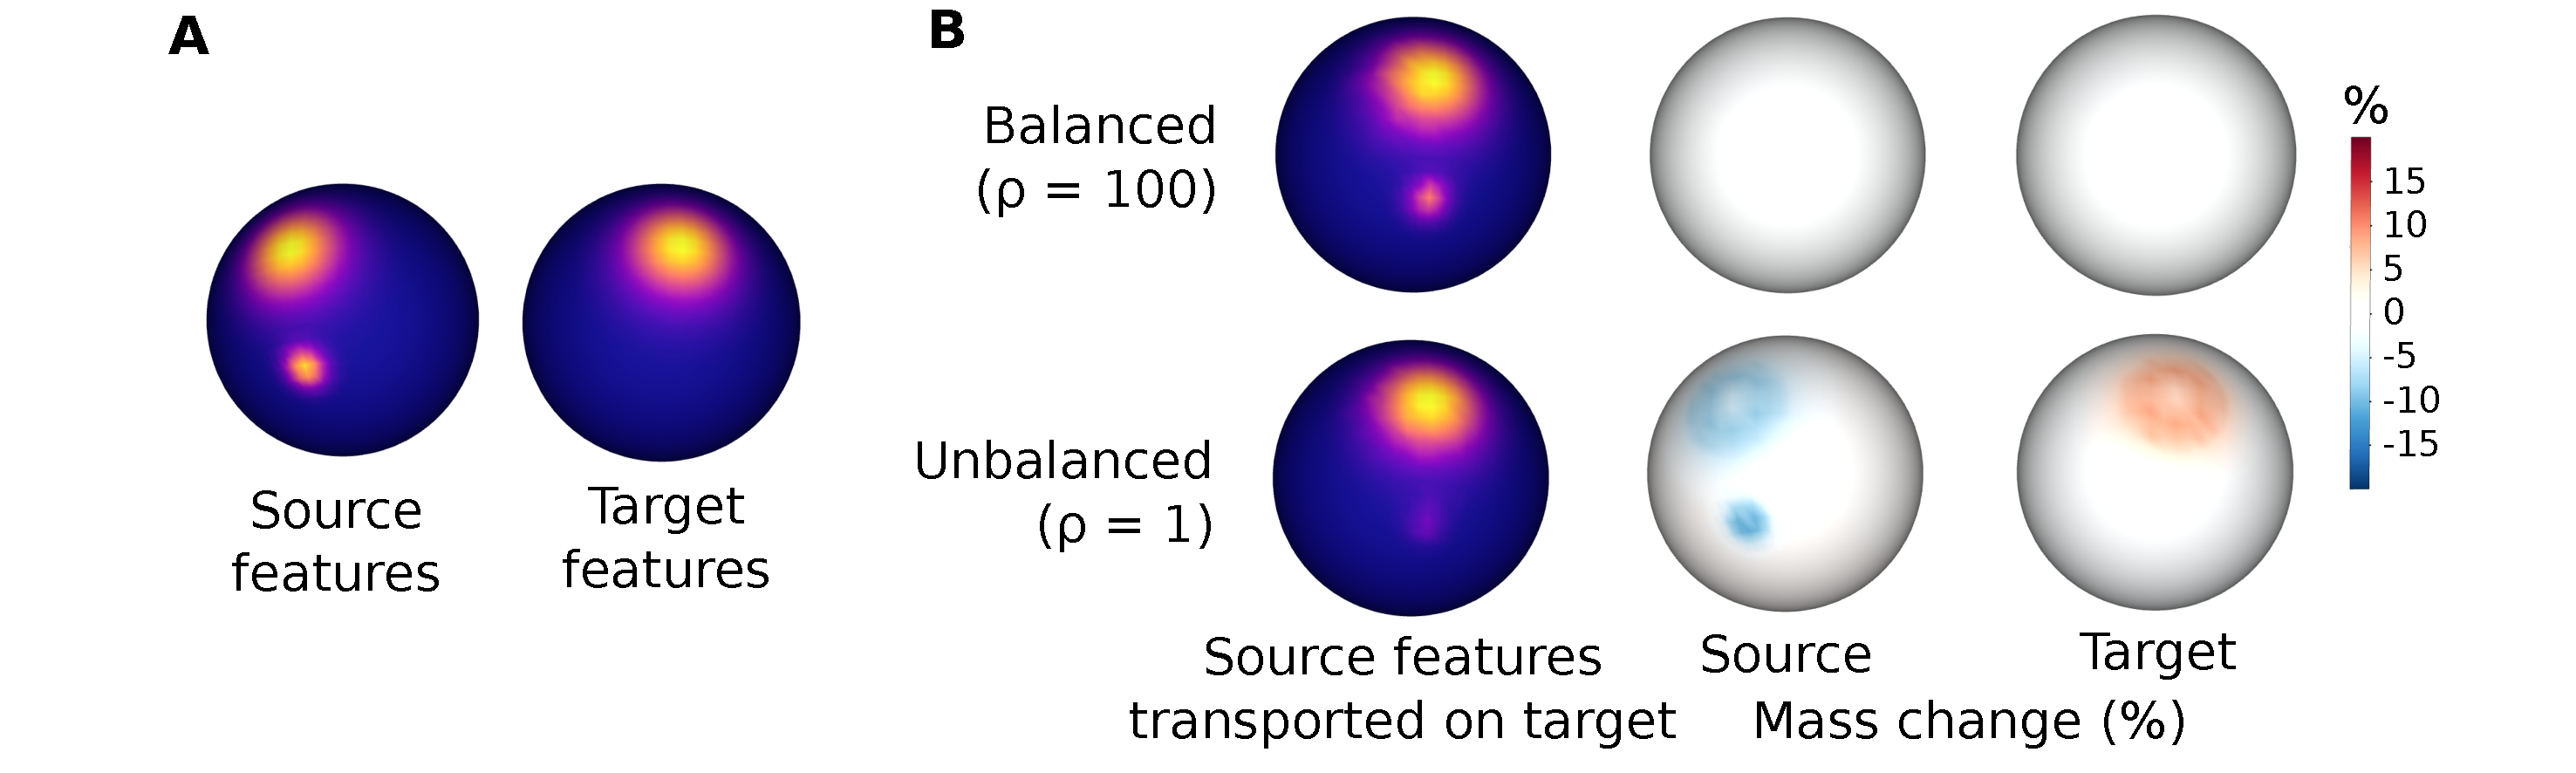
\includegraphics[width=1\columnwidth]{./Chapitre4/figures/toy_example.pdf}
    \caption{
        \textbf{Unbalancing helps accounting for idiosyncrasies of the source and target signals}
        When trying to align the source and target signals (Panel A),
        the classical balanced setup (Panel B, top row) transports all parts of
        the source signal even if they have no counterpart in the target signal.
        In the unbalanced setup (Panel B, bottom row), less source-only signal is transported:
        in particular, less mass is transported from the source's small blob onto the target
        (Panel B, middle column).
    }
    \label{fig:toy_example}
\end{figure}

%%%%%%%%%%%%%%%%%%%%%%%%%%%%%%%%%%%%%%%%%%
\subsubsection{Optimization}

Estimating the unbalanced Gromov Wasserstein loss is numerically sensitive to initialization,
due to the non-convexity of the problem.
Therefore, FUGW is also \textit{a priori} non-convex, and comparably difficult to estimate.
Consequently, following \citep{Sejourne20}, we instead compute a lower bound which
is formulated as a bi-convex problem that relies on the joint estimation of two couplings.
\begin{align}
    \label{eq:lbfugw}
    \quad \fugw(\cX^s, \cX^t) = \inf_{\substack{P, Q \geq 0 \\ P = Q}} L_{\theta}(P, Q)
    \geq \inf_{\substack{P, Q \geq 0 \\ m(P) = m(Q)}}
    L_{\theta}(P, Q) \triangleq \text{LB-FUGW} (\cX^s, \cX^t),
\end{align}
where $m(P) = \sum_{i,j} P_{i,j}$ denotes the mass of $P$ and
\begin{equation}
    \label{eq:fugw_loss_two_couplings}
    \begin{split}
        L_{\theta}(P, Q) \triangleq
        (1 - \alpha) \enspace L_{\text{W}}(P, Q) + \alpha \enspace L_{\text{GW}}(P, Q)
        + \rho \enspace L_{\text{U}}(P, Q) + \varepsilon \enspace E(P, Q),
    \end{split}
\end{equation}
where
\begin{itemize}
    \item[$\bullet$] $C \triangleq \Big( ||F^s_{i} - F^t_j||^2_2\Big)_{i,j} \in \bbR^2_+$ \hfill (feature cost matrix)

    \item[$\bullet$] $G \triangleq \Big( |D^s_{i,j} - D^t_{k,l}| \Big)_{i,j,k,l} \in \bbR^4_+$ \hfill (geometry cost matrix)

    \item[$\bullet$] $L_{\text{W}}(P, Q) \triangleq \langle C, \frac{P + Q}{2} \rangle = \frac{1}{2} ( \sum_{i,j} C_{i,j}P_{i,j} + \sum_{i,j} C_{i,j}Q_{i,j})$ \hfill (Wasserstein)

    \item[$\bullet$] $L_{\gw}(P, Q) \triangleq \langle G , P \otimes Q \rangle = \sum_{i,j,k,l}G_{i,j,k,l}P_{i,j}Q_{k,l}$ \hfill (Gromov-Wasserstein)

    \item[$\bullet$] $L_{\text{U}}(P, Q) \triangleq \enspace \kl \Big(P_{\# 1} \otimes Q_{\# 1} \vert w^s \otimes w^s \Big) + \enspace \kl \Big(P_{\# 2} \otimes Q_{\# 2} \vert w^t \otimes w^t \Big)$ \hfill (unbalancing)

    \item[$\bullet$] $E(P, Q) \triangleq \kl \Big(P \otimes Q | (w^s \otimes w^t) \otimes (w^s \otimes w^t) \Big)$ \hfill (entropy)
\end{itemize}
In particular, we have $L_{\theta}(P, P) = L_{\theta}(P)$,
which is the objective function of FUGW introduced in Equation \eqref{eq:fugw_obj_func}.
It is difficult to study when equality holds between FUGW and its lower bound.
Here, we attempt to understand the potential gap between them.
First, let us introduce the following problem
\begin{equation}
  \widetilde{\fugw}(\cX^s, \cX^t) = \inf_{(P, Q) \in \cE} L_{\theta}(P, Q),
\end{equation}
where $\cE = \{P, Q \geq 0: P_{\#1} = Q_{\#1}, P_{\#2} = Q_{\#2} \}$ is
the set of pairs of transportation plans whose corresponding marginal distributions are equal.
Clearly, we have
\begin{equation}
    \text{LB-FUGW} (\cX^s, \cX^t) \leq \widetilde{\fugw}(\cX^s, \cX^t)
    \leq \fugw(\cX^s, \cX^t).
\end{equation}
This inequality indicates that the difference between FUGW and LB-FUGW might be potentially large.
However, this gap can be tightened under the conditions in \Cref{prop:coot_gw_equiv}.
%%%%%%%%%%%%%%%%%%%%%%%%%%%%%%%%%%%%%%%%%%%%%
\begin{corollary} \label{coro:ugw_ucoot}
    If the distances $D^s$ and $D^t$ are of the forms: $D^s_{ij} = f_i + f_j + A_{ij}$ and
    $D^t_{kl} = g_k + g_l + B_{kl}$, where $f, g$ are vectors in $\bbR^n, \bbR^p$, respectively,
    and the matrices $A, B$ are both conditionally negative semi-definite, then we have
    $\fugw (\cX^s, \cX^t) = \widetilde{\fugw}(\cX^s, \cX^t)$.
    % Furthermore, if the definiteness holds, then the optimal solution satisfies $P^* = Q^*$,
    % meaning that $\text{LB-FUGW} (\cX^s, \cX^t) = \fugw(\cX^s, \cX^t)$.
\end{corollary}
%%%%%%%%%%%%%%%%%%%%%%%%%%%%%%%%%%%%%%%%%%%%%%%%
% In our experiments, while the geodesic distances do not necessarily meet these conditions,
In our experiments, while the geodesic distances do not necessarily meet these conditions,
we still observe that the two couplings of LB-FUGW are numerically equal.
So it is enough to choose, for example, the first one, as alignment between source and target signals.

The lower bound of FUGW involves solving a minimization problem with respect to two independent couplings:
Using a Block-Coordinate Descent (BCD) scheme, we fix a coupling and minimize
with respect to the other. This allows us to always be dealing with linear problems
instead of a quadratic one. Eventually, each BCD iteration consists in alternatively solving
two entropic unbalanced OT problems, whose solutions can be approximated using
the Sinkhorn algorithm \citep{Sejourne19}.

%%%%%%%%%%%%%%%%%%%%%%%%%%%%%%
\subsubsection{Barycenters}
Barycenters represent common patterns across samples.
Their role is instrumental in identifying a unique target for aligning a given group of individuals.
As seen in \Cref{fig:intro}, the vertex-wise group average does not usually provide
well-contrasted maps.
Inspired by the success of the GW distance when estimating the barycenter of structured objects
\citep{Peyre16,Vayer19b}, we use FUGW to find the barycenter
$(F_B, D_B) \in \bbR^{k \times c} \times \bbR^{k \times k}$
of all subjects $s \in \cS$, as well as the corresponding couplings $P^{s,B}$ from each subject
to the barycenter. More precisely, we solve
\begin{equation}
    \label{eq:barycenter}
    \cX^B = (F_B, D_B, w^B) \in \arg\min_{\cX}  \sum_{s \in \cS} \fugw(\cX^s, \cX),
\end{equation}
where we set the weights $w_B$ to be the uniform distribution.
By construction, the resulting barycenter benefits from the advantages of FUGW,
i.e. equilibrium between geometry-preserving and feature-matching properties,
while not forcing hard marginal constraints. The FUGW barycenter is estimated
using a Block-Coordinate Descent (BCD) algorithm that consists in alternatively
\textit{(i)} minimizing the OT plans $P^{s,B}$ for each FUGW computation
in \eqref{eq:barycenter} with fixed $\cX^B$ and \textit{(ii)}
updating the barycenter $\cX^B$ through a closed form with fixed $P^{s,B}$.
See \Cref{alg:fugw_barycenter} for more details.
The first step simply uses the previously introduced solver.
The second one takes advantage of the fact that the objective function introduced
in \eqref{eq:lbfugw} is differentiable in $F^B$ and $D^B$, and the two couplings of
LB-FUGW are numerically equal. This yields a closed form for $F^B$ and $D^B$,
as a function of $P^{s,B}$ and $\cX^s$. We note that, during the barycenter estimation,
the weight $w^B$ is always fixed as uniform distribution.

\begin{algorithm}[t]
    \caption{LB-FUGW barycenter for Problem \eqref{eq:barycenter}}
    \label{alg:fugw_barycenter}
    \begin{algorithmic}[1]
        \STATE \textbf{Input:} $(\cX^s)_{s \in \cS}, \rho, \alpha, \varepsilon$.
        \STATE \textbf{Output:} Individual couplings $(P^{s, B})_{s \in \cS}$, barycenter $\cX^B$.
        \STATE Initialize: $F^B = \mathbb I_k$; $D^B = 0_k$.
        \WHILE{$\cX^B = (F^B, D^B, w^B)$ has not converged}
            \STATE Draw $\widetilde{S}$ subset of $S$.
            \FOR{$s \in \widetilde{S}$}
                \STATE Align: $P^{s, B} \gets \text{LB-FUGW}(\cX^s, \cX^B, \rho, \alpha, \varepsilon)$.
                \COMMENT{Fixed $\cX^B$}
            \ENDFOR
            \STATE Update $F^B$, $D^B$:
            \COMMENT{Fixed $P^{s, B}$}
            \begin{equation*}
                F^B = \frac{1}{| \widetilde{S} |} \sum_{s \in \widetilde{S}}
                \text{diag} \left( \frac{1}{P^{s, B}_{\# 2}} \right)
                (P^{s, B})^\top F^s \; \text{ and } \;
                D_B = \frac{1}{| \widetilde{S} |} \sum_{s \in \widetilde{S}}
                \frac{(P^{s, B})^\top D^s P^{s, B}}{P^{s, B}_{\# 2} (P^{s, B}_{\# 2})^\top}.
            \end{equation*}
        \ENDWHILE
    \end{algorithmic}
\end{algorithm}

%%%%%%%%%%%%%%%%%%%%%%%%%%%%%%%%%%%%%%%%%ù
\subsection{Numerical experiments}

We design three experiments to assess the performance of FUGW.
In Experiments 1 and 2, we are interested in assessing if aligning pairs of individuals with
FUGW increases correlation between subjects compared to a baseline correlation.
We also compare the ensuing gains with those obtained when using the
competing method MSM \citep{robinson_msm_2014,robinson_multimodal_2018} to align subjects.
In Experiment 3, we derive a barycenter of individuals and assess its ability to capture fine-grained
details compared to classical methods.

\paragraph{Dataset}
\label{par:dataset}
In all three experiments, we leverage data from the Individual Brain Charting dataset \citep{ibc}.
It is a longitudinal study on 12 human subjects,
comprising 400 fMRI maps per subject collected
on a wide variety of stimuli (motor, visual, auditory, theory of mind,
language, mathematics, emotions, and more), movie-watching data, T1-weighted maps, as well as other features such as
retinotopy which we don't use in this work. We leverage these 400 fMRI maps.
The training, validation and test sets respectively comprise
326, 43 and 30 contrast maps acquired for each individual of the dataset.
Tasks and MRI sessions differ between each of the sets.
% More details, including preprocessing, are provided in Supplementary Materials.

\paragraph{Baseline alignment correlation}
For each pair of individuals $(s, t)$ under study, and for each fMRI contrast $c$ in the test set,
we compute the Pearson correlation $\text{corr}(F^s_{\cdot, c}, F^t_{\cdot, c})$
after these maps have been projected onto a common surface anatomy (in this case, \emph{fsaverage5}
mesh). Throughout this work, such computations are made for each hemisphere separately.

\paragraph{Experiment 1 - Aligning pairs of humans with the same anatomy}
%
For each pair $(s, t)$ under study, we derive an alignment $P^{s,t} \in \bbR^{n \times p}$
using FUGW on a set of training features. In this experiment, source and target data
lie on the same anatomical mesh (\emph{fsaverage5}), and $n = p = 10240$ for each hemisphere.
Since each hemisphere's mesh is connected, we align one hemisphere at a time.

Computed couplings are used to align contrast maps of a the validation set from
the source subject onto the target subject. Indeed, one can define
$\phi_{s \rightarrow t} \colon X \in \bbR^{n \times q}
\mapsto \big((P^{s,t})^T X \big) \oslash P^{s,t}_{\#2} \in \bbR^{p \times q}$
where $\oslash$ represents the element-wise division. $\phi_{s \rightarrow t}$
transports any matrix of features from the source mesh to the target mesh.
We measure the Pearson correlation $\text{corr}\big( \phi_{s \rightarrow t}(F^s), F^t \big)$
between each aligned source and target maps.

We run a similar experiment for MSM and compute the correlation gain induced on a
test set by FUGW and MSM respectively.
For both models, we selected the hyper-parameters maximizing correlation gain on a validation set.
In the case of FUGW, in addition to gains in correlation, hyper-parameter selection
was influenced by three other metrics that help us assess the relevance of computed couplings:

\begin{description}
    \item[Transported mass]
    For each vertex $i$ of the source subject, we compute
    $\sum \limits_{0 \leq j < p} P^{s,t}_{i, j}$.

    \item[Vertex displacement]
    Taking advantage of the fact that the source and target anatomies are the same,
    we define $D = D^s = D^t$ and compute for each vertex $i$ of the source subject the quantity
    $\sum_j P^{s,t}_{i, j} \cdot D_{i, j} / \sum_j P^{s,t}_{i,j}$,
    which measures the average geodesic distance on the cortical sheet between vertex $i$
    and the vertices of the target it has been matched with.

    \item[Vertex spread]
    Large values of $\varepsilon$ increase the entropy of derived couplings.
    To quantify this effect, and because we don't want the matching to be too blurry,
    we assess how much a vertex was \textit{spread}. Considering
    $\tilde{P_i} = P^{s,t}_i / \sum_j P^{s,t}_{i,j} \in \bbR^p$
    as a probability measure on target vertices,
    we estimate the anatomical variance of this measure by sampling $q$ pairs
    $(j_q, k_q)$ of $\tilde{P_i}$ and computing their average geodesic distance
    $\frac{1}{q} \sum\limits_{j_q, k_q} D_{j_q, k_q}$.
\end{description}

\paragraph{Experiment 2 - Aligning pairs of humans with individual anatomies}
We perform a second alignment experiment, this time using individual meshes instead of
an anatomical template. Importantly, in this case,  there is no possibility to compare
FUGW with baseline methods, since those cannot handle this case.
However, individual meshes are significantly larger than the
common anatomical template used in Experiment 1 ($n \approx m \approx$ 160k vs. 10k previously),
resulting in couplings too large to fit on GPUs -- for reference,
a coupling of size 10k $\times$ 10k already weights ~400Mo on disk.
We thus reduce the size of the source and target data by
clustering them into 10k small connected clusters using Ward's algorithm \citep{thirion:2014}.
% More details are given in supplementary section A.4.

\paragraph{Experiment 3 - Comparing FUGW barycenters with usual group analysis}
\label{par:barycenter}

Since it is very difficult to estimate the barycentric mesh, we force it to be equal to
the \emph{fsaverage5} template. Empirically, this we force the distance matrix $D^B$
to be equal to that of \emph{fsaverage5}, and only estimate the functional barycenter $F^B$.
We initialize it with the mean of $(F^s)_{s \in S}$
and derive $F^B$ and $(P^{s,B})_{s \in S}$ from Problem \eqref{eq:barycenter}.
Then, for a given stimulus $c$, we compute its projection onto the barycenter for each subject.
We use these projections to compute two maps of interest:
\textit{(i)} $M_{B,c}$ the mean of projected contrast maps across subjects
and \textit{(ii)} $T_{B,c}$ the t-statistic (for each vertex) of projected maps.
We compare these two maps with their unaligned counterparts $M_{0,c}$ and $T_{0,c}$ respectively.
\begin{figure}[ht]
    \begin{minipage}{.4\linewidth}
        \begin{equation*}
            M_{B,c} \triangleq \frac{1}{|S|} \sum_{s \in S} \phi_{s \rightarrow t}(F^s_{\cdot, c})
        \end{equation*}
    \end{minipage}
    \hfil
    \begin{minipage}{.5\linewidth}
        \begin{equation*}
            T_{B,c} \triangleq \text{t-statistic} \Big( \big(
                \phi_{s \rightarrow t}(F^s_{\cdot, c}) \big)_{s \in S} \Big)
        \end{equation*}
    \end{minipage}
\end{figure}
% \vspace*{-0.5\baselineskip}
\begin{figure}[ht]
    \begin{minipage}{.4\linewidth}
        \begin{equation*}
            M_{0,c} \triangleq \frac{1}{|S|} \sum_{s \in S} F^s_{\cdot, c}
        \end{equation*}
    \end{minipage}
    \hfil
    \begin{minipage}{.5\linewidth}
        \begin{equation*}
            T_{0,c} \triangleq \text{t-statistic} \Big( (F^s_{\cdot, c})_{s \in S} \Big)
        \end{equation*}
    \end{minipage}
\end{figure}
The first map helps us to qualitatively evaluate the precision of FUGW alignments and barycenter.
The second one is classically used to infer the existence of areas of the brain that
respond to specific stimuli. We assess whether FUGW helps find the same clusters of vertices.
Eventually, we quantify the number of vertices significantly activated or deactivated
with and without alignment respectively.

\subsection{Results}

\subsubsection{Experiment 1 - Template anatomy}

\paragraph{Aligning subjects on a fixed mesh}

We set $\alpha = 0.5$, $\rho = 1$ and $\varepsilon = 10^{-3}$.
Pearson correlation between source and target contrast maps is systematically and
significantly increased when aligned using FUGW, as illustrated in
\Cref{fig:gain_comparisions_fsaverage5} where correlation grows by almost $40\%$
from $0.258$ to $0.356$.

\begin{figure}[ht!]
    \centering
    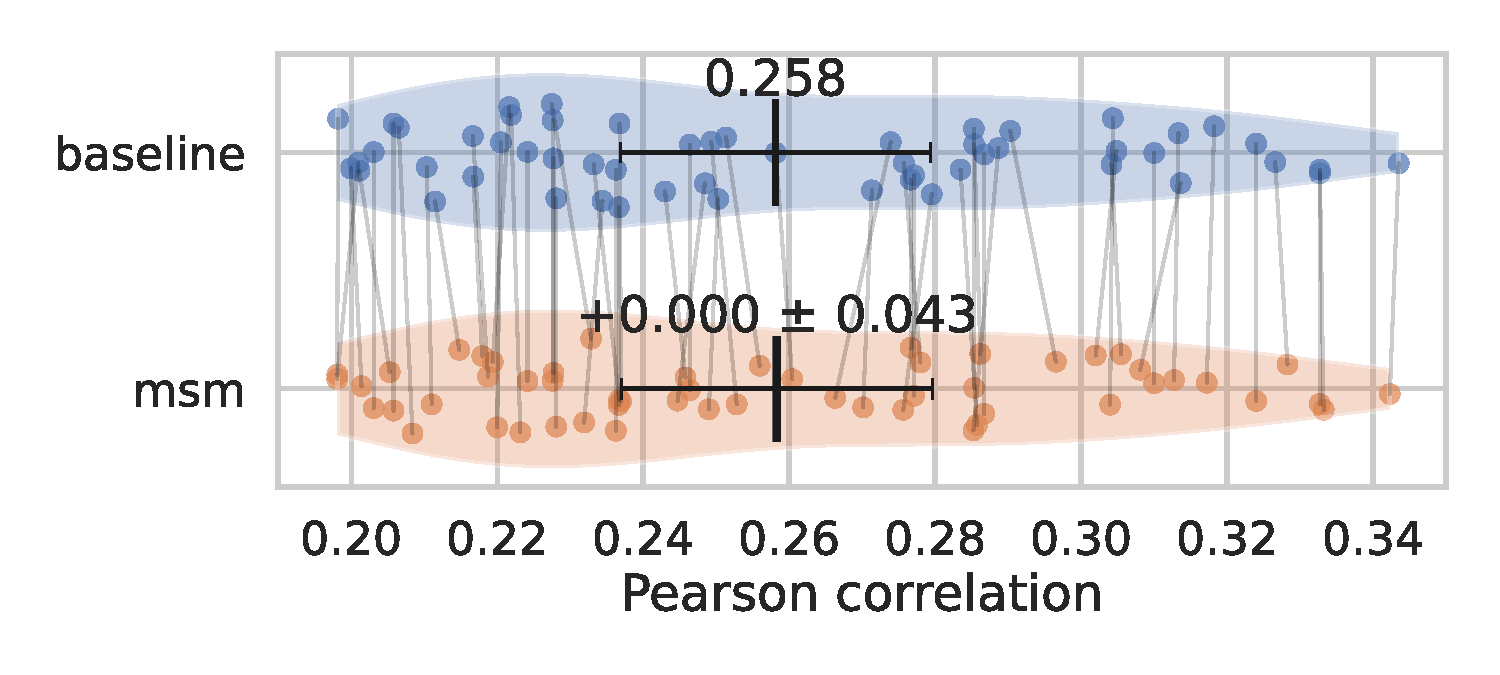
\includegraphics[width=0.49\columnwidth]{./Chapitre4/figures/fsaverage5_alignment_correlation_gain_msm.pdf}
    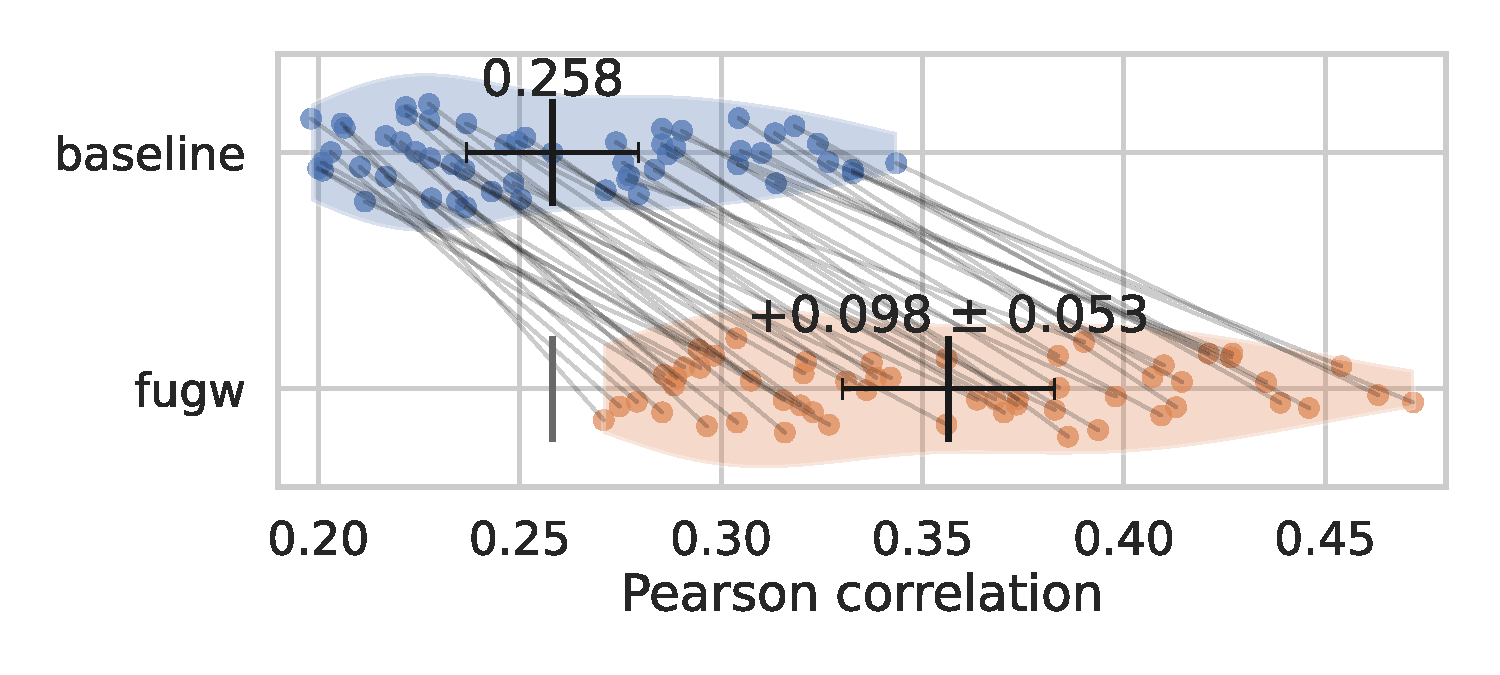
\includegraphics[width=0.49\columnwidth]{./Chapitre4/figures/fsaverage5_alignment_correlation_gain_fugw.pdf}
    \caption{
        \textbf{Comparison of gains in correlation after inter-subject alignment}
        For each pair of source and target subjects of the dataset,
        we compute the average Pearson correlation between 30 test contrasts,
        leading to the (baseline) correspondence score,
        and compare it with that of the same contrast maps
        aligned with either MSM (left) or FUGW (right). Correlation gains are much better for FUGW.
    }
    \label{fig:gain_comparisions_fsaverage5}
\end{figure}
% We also varied training sets by selecting subsets of training contrasts and find that
% similar performance on the test set can be achieved regardless of the training data
% (see Supplementary \Cref{sec:control_experiments} and in particular Supplementary
% \Cref{tab:varying_training_sets}).

\paragraph{Hyper-parameters selection}
\label{par:params_selection}

Hyper-parameters used to obtain these results were chosen
after running a grid search on $\alpha$, $\varepsilon$ and $\rho$
and evaluating it on the validation dataset.
Computation took about 100 hours using 4 Tesla V100-DGXS-32GB GPUs. More precisely,
it takes about 4 minutes to compute one coupling between a source and target 10k-vertex
hemisphere on a single GPU, when the solver was set to run 10 BCD and 400 Sinkhorn iterations.
In comparison, MSM takes about the same time on Intel(R) Xeon(R) CPU E5-2698 v4 @ 2.20GHz CPUs.
Results are reported in \Cref{fig:cv_metrics} and provide multiple insights concerning FUGW.

Firstly, without anatomical constraint ($\alpha = 0$),
source vertices can be matched with target vertices
that are arbitrarily far on the cortical sheet.
Even though this can significantly increase correlation, it also
results in very high vertex displacement values (up to $100mm$).
Such couplings are not anatomically plausible.
%
Secondly, without functional information ($\alpha = 1$),
couplings recover a nearly flawless matching between source and target meshes,
so that, when $\varepsilon = 10^{-5}$
(ie when we force couplings to find single-vertex-to-single-vertex matches),
vertex displacement and spread are close to 0 and correlation is unchanged.
%
Fusing both constraints ($0 < \alpha < 1$)
yields the largest gains in correlation while allowing to compute
anatomically plausible reorganizations the cortical sheet between subjects.

The impact of $\rho$ (controlling marginal penalizations) on correlation seems modest,
with a slight tendency of increased correlation in unbalanced problems (low $\rho$).

Finally, it is worth noting that a relatively wide range of $\alpha$ and $\rho$ yield comparable gains.
The fact that FUGW performance is weakly sensitive to hyper-parameters makes it
a good off-the-shelf tool for neuroscientists who wish to derive inter-individual alignments.
However, $\varepsilon$ is of dramatic importance in computed results and should be chosen carefully.
Vertex spread is a useful metric to choose sensible values of $\varepsilon$;
for human data one might consider that it should not exceed $20mm$.

\begin{figure}[ht]
    \centering
    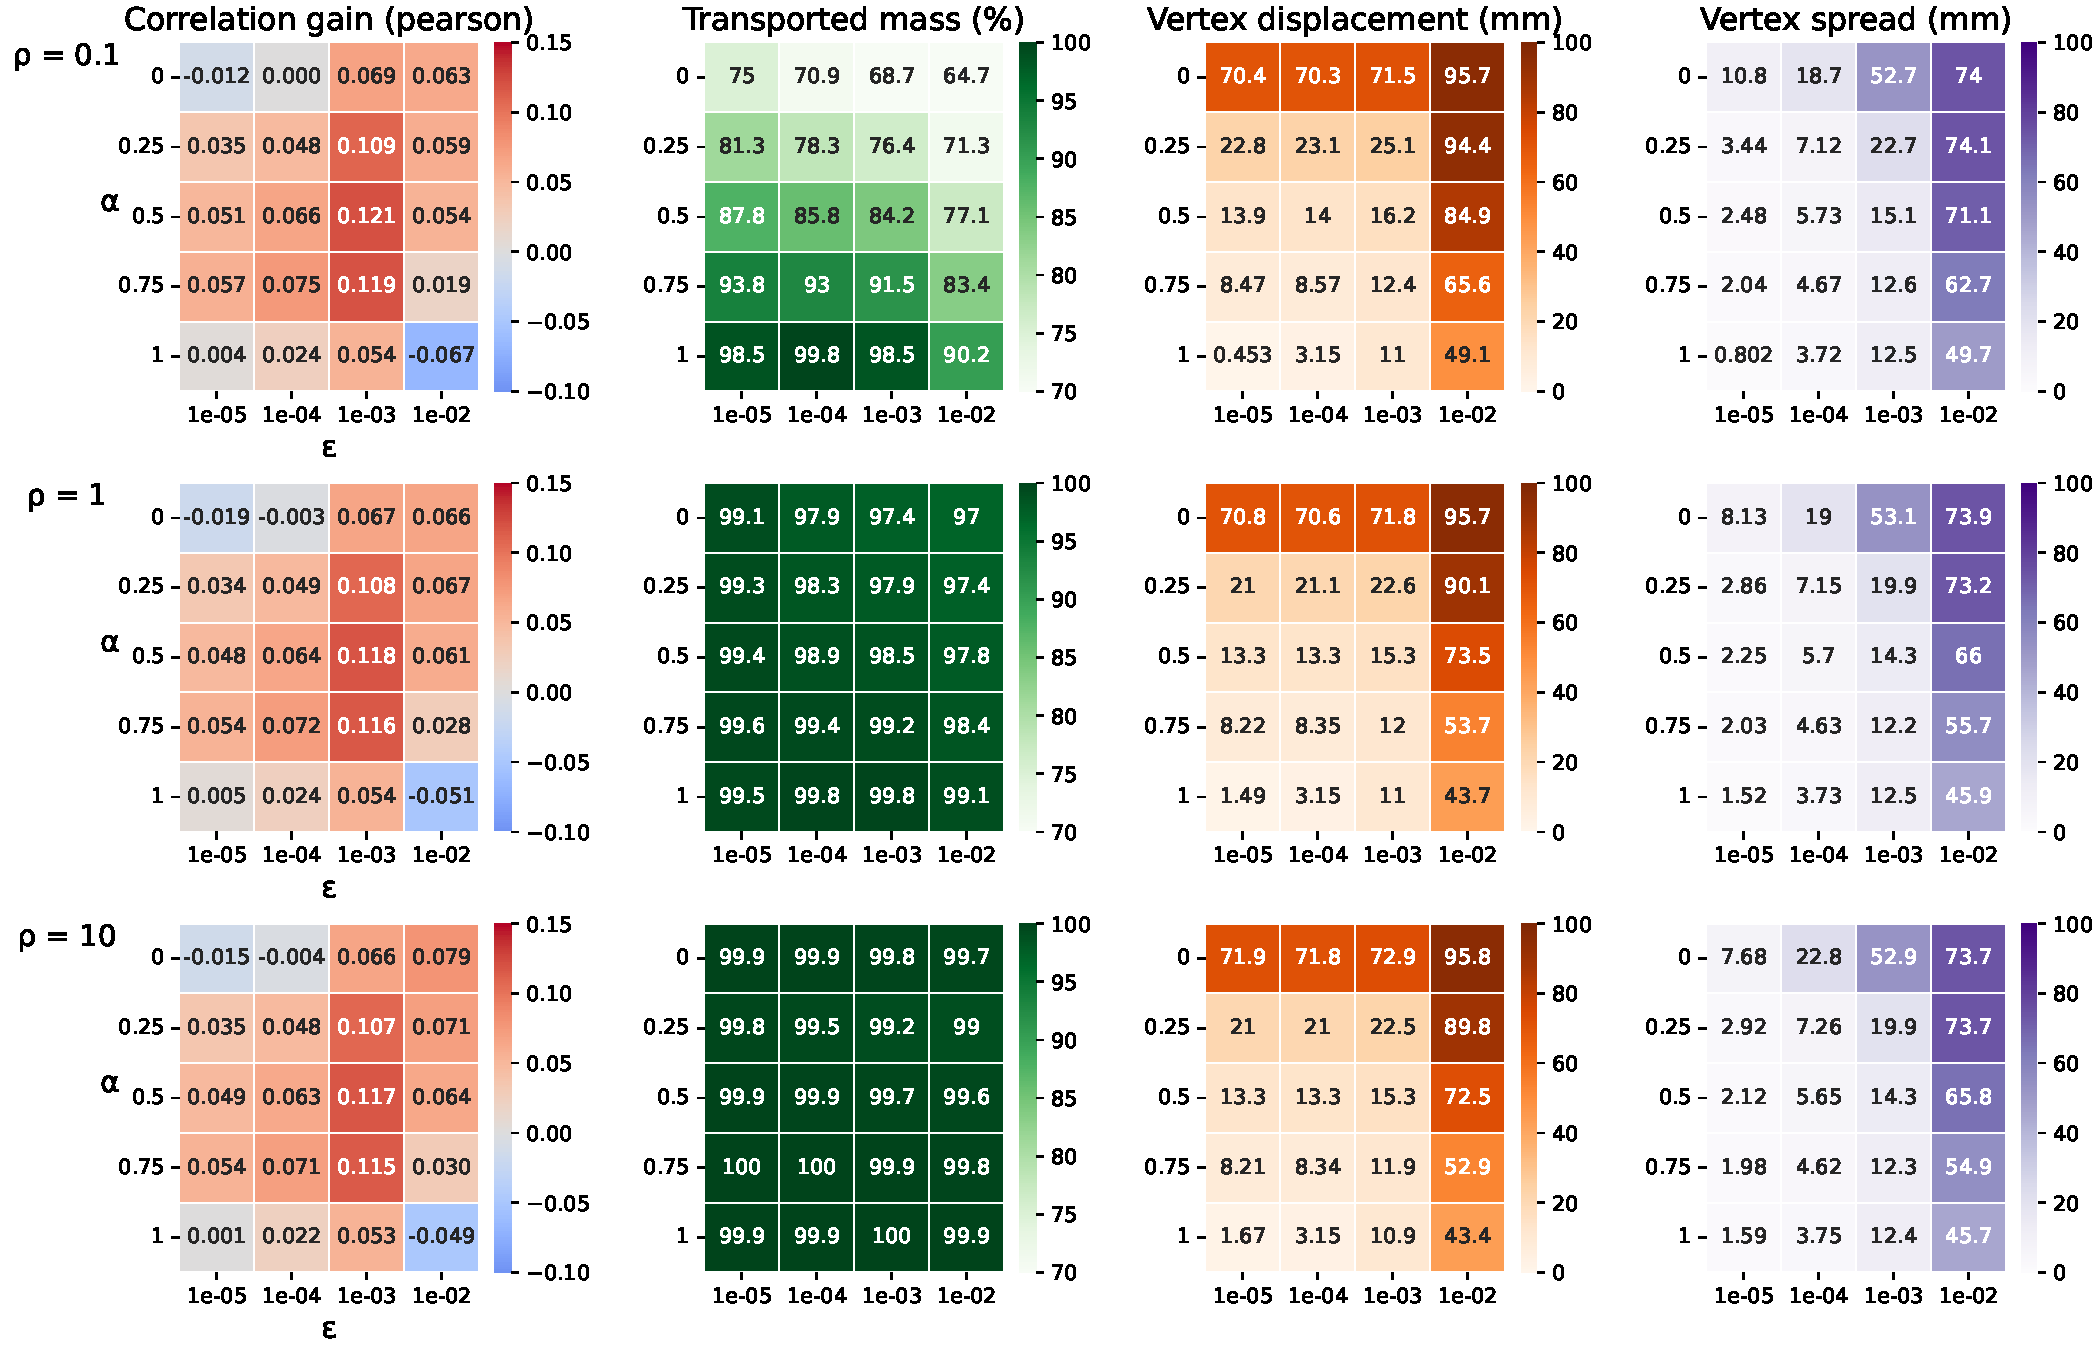
\includegraphics[width=1\columnwidth]{./Chapitre4/figures/cv_all_metrics_hcp_left_fugw.pdf}
    \caption{
        \textbf{Exploring hyper-parameter space to find relevant couplings}
        Given a transport plan aligning a source and target subject,
        we evaluate how much this coupling
        (left) improves correlation between unseen contrast maps
        of the two subjects,
        (center left) actually transports data,
        (center right) moves vertices far from their original location on the cortical surface
        and (right) spreads vertices on the cortical sheet.
        We seek plans that maximize correlation gain, while keeping spread and displacement low enough.
    }
    \label{fig:cv_metrics}
\end{figure}

\paragraph{Mass redistribution in unbalanced couplings}
Unbalanced couplings provide additional information about how functional areas might differ
in size between pairs of individuals. This is illustrated in \Cref{fig:transported_mass},
where we observe variation in size of the auditory area between a given pair of individuals.
This feature is indeed captured by the difference of mass between subjects
(although the displayed contrast was not part of the training set).
\begin{figure}[!th]
    \centering
    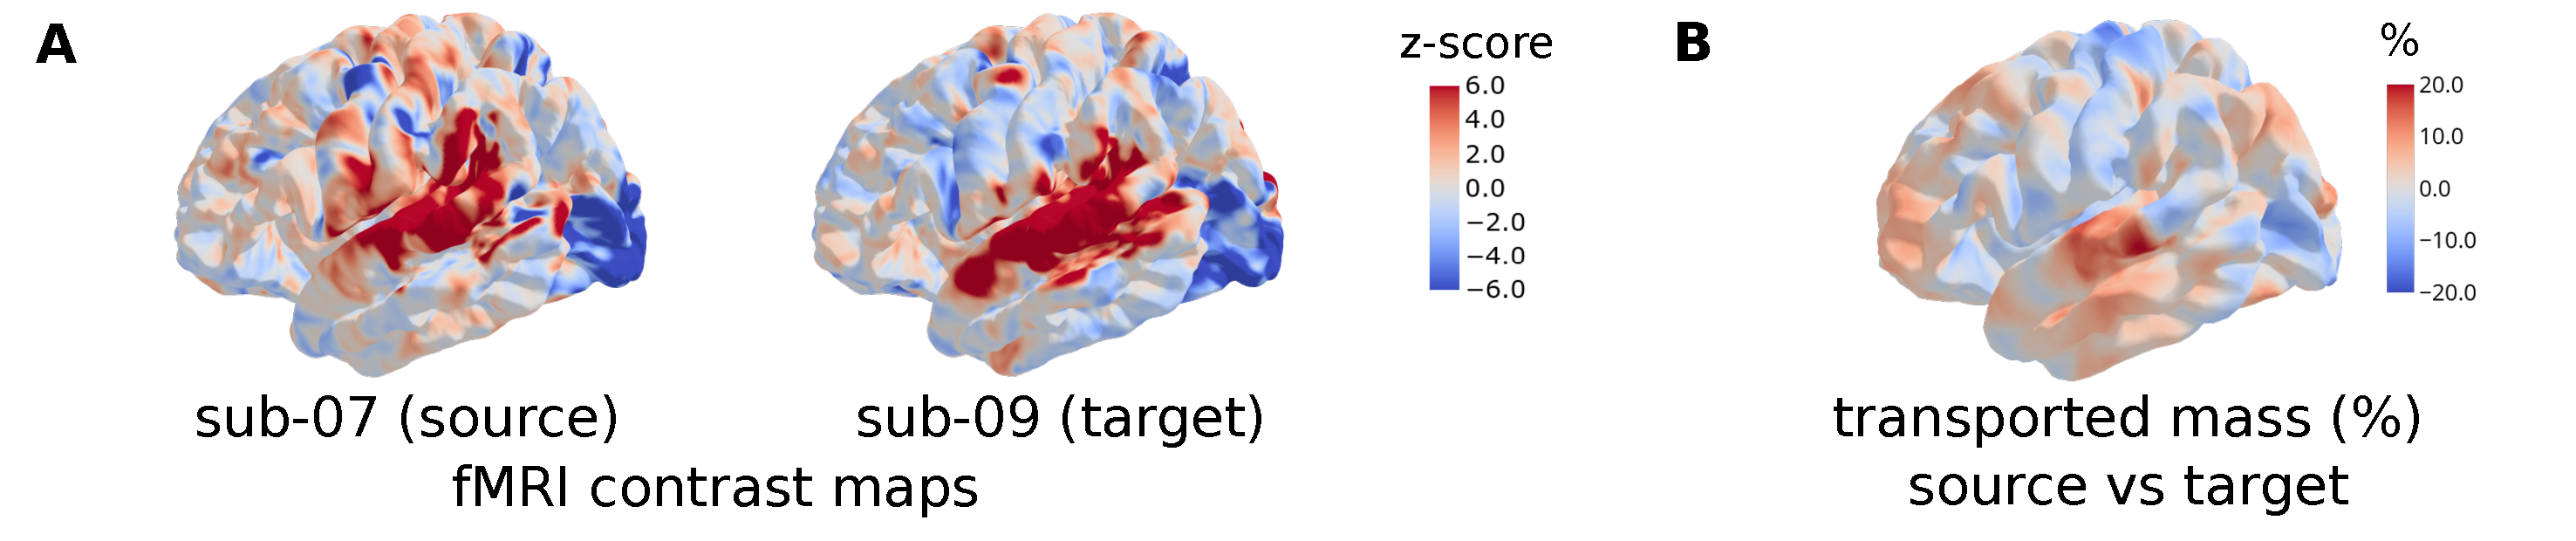
\includegraphics[width=1\columnwidth]{./Chapitre4/figures/transported_mass.pdf}
    \caption{
        \textbf{Transported mass indicates areas which have to be resized between subjects}
        (Panel A) We show a contrast map from the test set which displays areas showing
        stronger activation during auditory tasks versus equivalent visual tasks. It shows much more
        anterior activations on the target subject compared to the source subject.
        This is consistent with the observation that more mass is present in
        anterior auditory areas of the source subject than in the target subject (Panel B).
    }
    \label{fig:transported_mass}
\end{figure}

\subsubsection{Experiment 2 - Individual anatomies}
\begin{figure}[!ht]
    \centering
    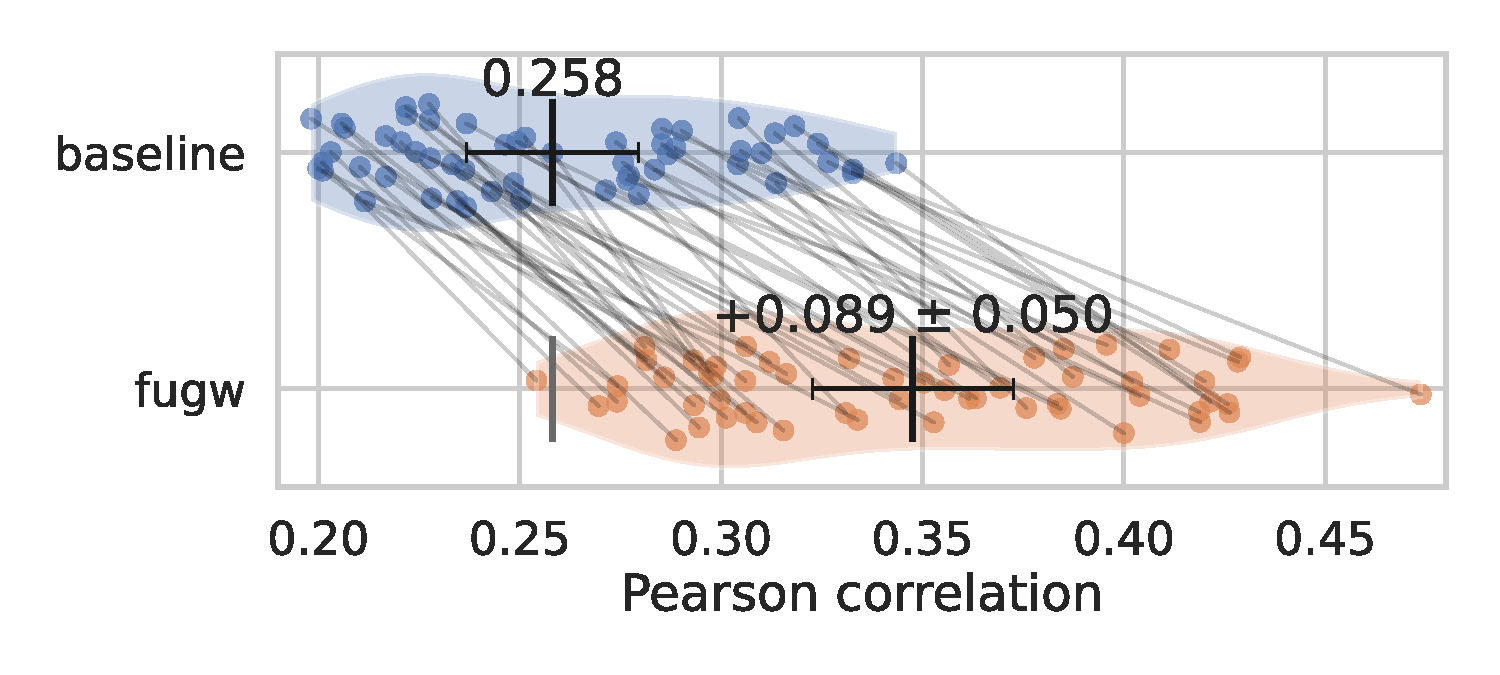
\includegraphics[width=0.5\columnwidth]{./Chapitre4/figures/individual_alignment_correlation_gain_fugw}
    \caption{
        \textbf{Correlation between pairs of subjects is significantly better after alignment on individual anatomies than after projecting subjects onto a common anatomical template}
    }
    \label{fig:gain_comparisions_individual}
\end{figure}

As shown in \Cref{fig:gain_comparisions_individual},
we obtain correlation gains which are comparable to that of Experiment 1 (about 35\% gain)
while working on individual meshes.
This tends to show that FUGW can compute meaningful alignments between pairs of individuals
without the use of an anatomical template, which helps bridge most conceptual impediments listed
in \Cref{sec:introduction}.
Moreover, this opens the way for computation of simple statistics in cohorts of individuals
in the absence of a template. Indeed, one can pick an individual of the cohort and use it
as a reference subject on which to transport all other individuals.
We give an example in \Cref{fig:individual_projections},
showing that FUGW correctly preserved idiosyncrasies of each subject while
transporting their functional signal in an anatomically sound way.
\begin{figure}[H]
    \centering
    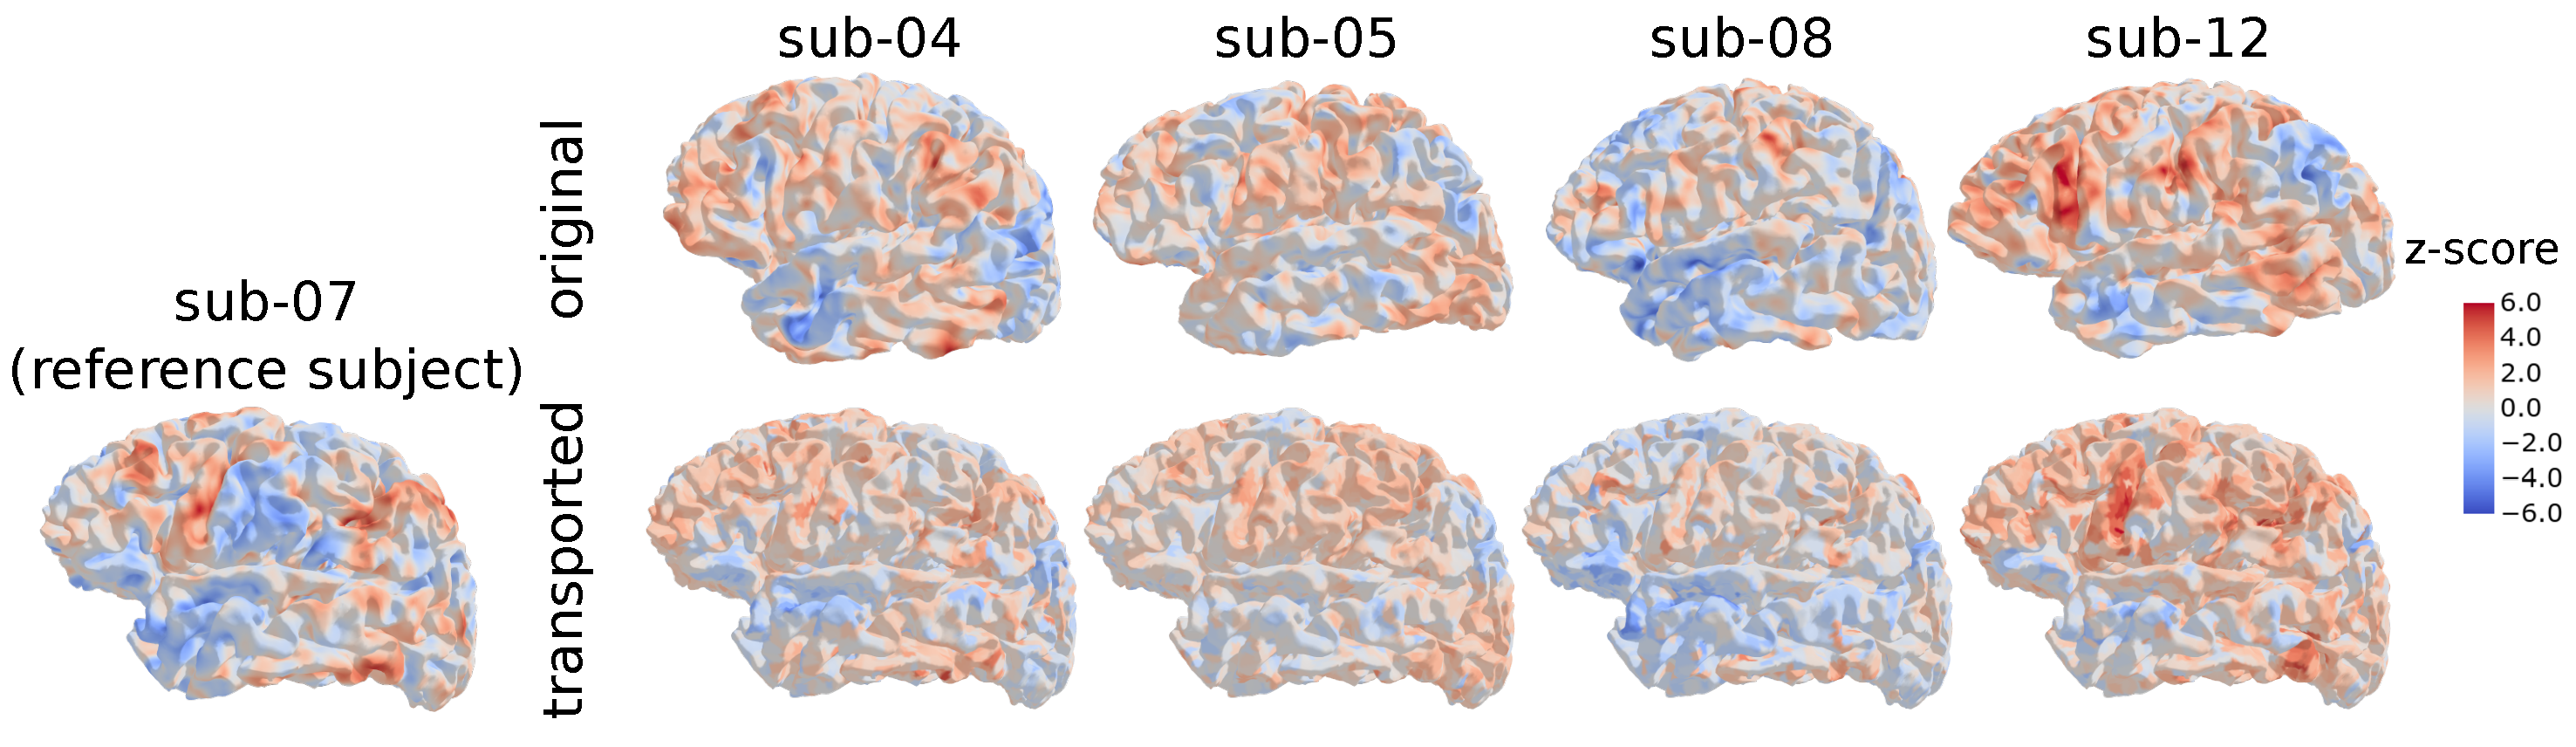
\includegraphics[width=1\columnwidth]{./Chapitre4/figures/individual_alignment.pdf}
    \caption{
        \textbf{Transporting individual maps onto a reference subject}
        FUGW can help bridge the absence of template anatomies
        and derive pairs of alignments such that all individuals
        of the cohort are comparable. We display a map taken from the test set contrasting areas activated during mathematical reasoning against areas activated for other stimuli of the protocol.
    }
    \label{fig:individual_projections}
\end{figure}

\subsubsection{Experiment 3 - Barycenter}

In the absence of a proper metric to quantify the correctness of a barycenter,
we first qualitatively compare the functional templates obtained with and without alignment.
In \Cref{fig:barycenter_vs_group_average}.A, we do so using brain maps taken from the test set.
We can see that the barycenter obtained with FUGW yields sharper contrasts and
more fine-grained details than the barycenter obtained by per-vertex averaging.
We also display in \Cref{fig:barycenter_vs_group_average}.B
the result of a one-sample test for the same contrast, which can readily be used for inference.
The one-sample test map obtained after alignment to the FUGW template exhibits
the same supra-threshold clusters as the original approach, but also some additional spots
which were likely lost due to inter-subject variability in the \emph{fsaverage5} space.
This approach is thus very useful to increase power in group inference.
We quantify this result by counting the number of supra-threshold vertices
with and without alignment for each contrast map of the test set.
Our alignment method significantly finds more such vertices of interest,
as shown in \Cref{fig:barycenter_vs_group_average}.C.
\begin{figure}[t]
    \centering
    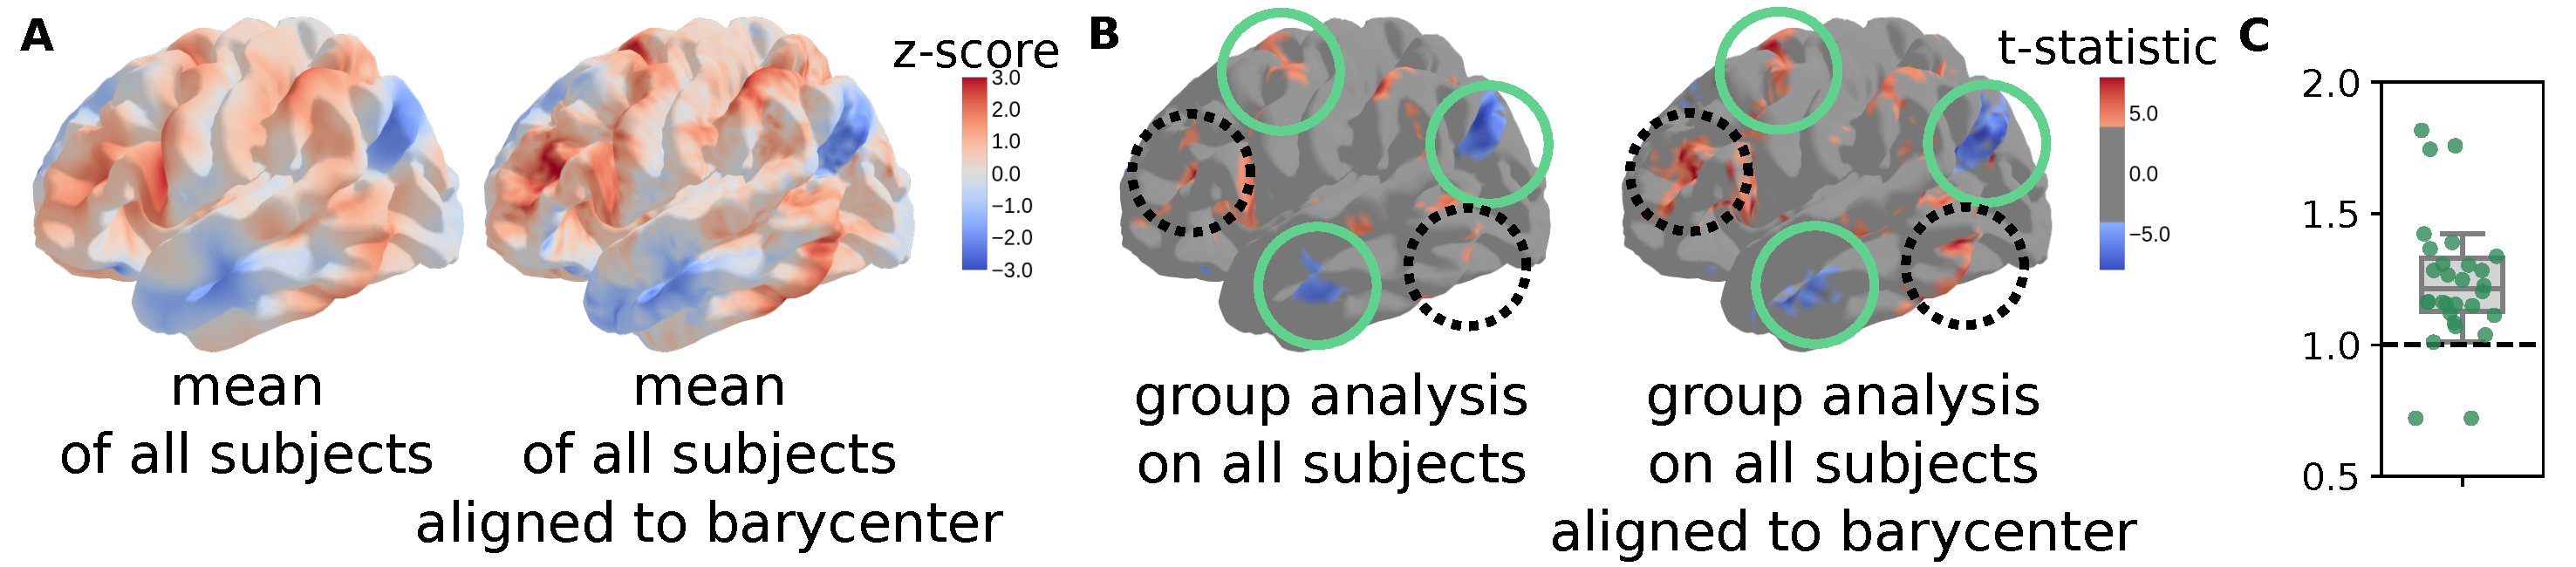
\includegraphics[width=1\columnwidth]{./Chapitre4/figures/barycenter_group_analysis.pdf}
    \caption{
        \textbf{FUGW barycenter yields much finer-grained maps than group averages}
        We study the same statistical map as in \Cref{fig:intro}, which contrasts
        areas of the brain involved in mathematical reasoning.
        \textbf{A}. These complex maps projected onto the barycenter and averaged
        show more specific activation patterns than simple group averages,
        especially in cortical areas exhibiting more variability, such as the prefrontal cortex.
        \textbf{B}. Deriving a t-test on aligned maps captures the same clusters
        as the classical approach (plain green circles), but also new clusters in areas
        where inter-subject variability is high (dotted black circles).
        Peak t-statistics are also higher with FUGW.
        \textbf{C}. Ratio of number of activated vertices ($|\text{t-statistic}| \geq 4$)
        with versus without alignment for each map of the test set.
        Our method finds significantly more of such vertices ($\text{p-value} = 3\cdot10^{-4}$).}
    \label{fig:barycenter_vs_group_average}
\end{figure}

\subsection{Discussion}

FUGW can derive meaningful couplings between pairs of subjects without
the need of a pre-existing anatomical template. It is well-suited to computing
barycenters of individuals, even for small cohorts.

In addition, we have shown clear evidence that FUGW yields gains that cannot be achieved
by traditional diffeomorphic registration methods.
These methods impose very strong constraints to the displacement field,
that may prevent reaching optimal configurations.
More deeply, this finding suggests that brain comparison ultimately requires
lifting hard regularity constraints on the alignment models,
and that two human brains differ by more than a simple continuous surface deformation.
However, current results have not shown a strong correlation gain of
unbalanced OT compared to balanced OT, likely because the cohort under study is too small.
Leveraging datasets such as HCP \citep{hcpdata} with a larger number of subjects
will help lower the standard error on correlation gain estimates.
In this work, we decided to rely on a predefined anatomical template (\emph{fsaverage5})
to derive functional barycenters.
It would be interesting to investigate whether more representative anatomical templates
can be learned during the process.
This would in particular help to customize templates to different populations or species.

Additionally, using an entropic solver introduces a new hyper-parameter $\varepsilon$
that has a strong effect, but is hard to interpret.
Future work may replace the Sinkhorn algorithm \citep{Sejourne19}
used here by the majorization-minimization one \citep{Chapel20},
which does not require entropic smoothing. This solution can yield sparse couplings
while being orders of magnitude faster, which will prove useful when computing barycenters
on large cohorts.

Finally, we plan to make use of FUGW to derive alignments between human and
non-human primates without anatomical priors. Indeed, the understanding of given brain mechanisms
will benefit from more detailed invasive measurements made on other species \emph{only if}
brains can be matched across species; moreover, this  raises the question of features
that make the human brain unique, by identifying patterns that have no counterpart in other species.
By maximizing the functional alignment between areas, but also allowing for some regions
to be massively shrunk or downright absent in one species relative to the other,
the present tool could shed an objective light on the important issue of whether
and how the language-related areas of the human cortical sheet map onto
the architecture of non-human primate brains.

\vfill